\chapter{Fusion Enriched Hypergraph Linguistic Model}
\label{chap:ling_net}
\begin{abstractchap}
In the previous chapter we presented the theoretical notions used to represent text with a distributional approach, that is, the parameters, the models to implement them  and the problems that naturally arise from these kinds of representations. In this chapter we introduce and define the first set of our contributions. Briefly, we present a linguistic framework to represent textual data. Feature fusion techniques are then applied over this network in order to better leverage the data contained in it while addressing the sparsity issue.

We organize this  chapter  in four parts: we present a brief state of the art on how the information contained in linguistic graphs is used for WSD/WSI and NER. Secondly, we introduce our model. Thirdly, we present  the method used to combine the data held in our mode, specifically using feature fusion techniques. Finally, we materialize the proposed model by transforming an English Wikipedia based corpus into our proposed framework.
\end{abstractchap}
\minitoc

\section{Introduction}

In the previous chapter we covered the details concerning the parameters regarding the construction of a distributional representation model, as well as its challenges.
The challenges that we will address in this chapter are two: (1) how to organize heterogeneous textual information within a single linguistic resource, and (2), how to leverage said information to obtain complementary representation spaces, while taking into account the feature sparsity issue that is characteristic of textual data.


The first two contributions of this thesis are contained in a fusion enriched hypergraph linguistic model proposition. The model consists on two components which address two research questions each: the issue of making sparsity less severe and leveraging different types of features  by using a single feature representation space. We will describe our motivations and its characteristics in the following paragraphs. We can see the block diagram of the ensemble of our propositions  on Figure \ref{fig:maindiag}. There, we can observe our enriched linguistic model proposition, comprising our first two propositions, which is the focus of this chapter, as well as the instantiation of said model using a Wikipedia based corpus. %On the bottom, we show the application of said model in NLP tasks, described thoroughly in Chapter \ref{chap:wsd}.

The model we present here entails three  important characteristics: firstly, the possibility to leverage different\footnote{We use three in our model definition: syntactic, lexical  and what we will call standard features (explained later on).} types of information.  Secondly, as the words will be linked together, there is an inner structure that will emerge from the model and which we exploit in our experiments. Thirdly, given that we treat unstructured text data, the relations (or features)  between words are sparse, this is alleviated by combining features via fusion techniques.  The three of them are addressed with our propositions. 
In the following chapter, we test the practicality of our proposal with well-established tasks and related evaluation corpora, which we use as benchmark input data in our experiments. 

Our network is based on the distributional hypothesis, as described in the previous chapter.  As co-occurrence features, we select both lexical and syntactic contexts, indeed creating a linguistic resource that hold both types of information in order to get a complementary insight of words' relations. Our network sets a lexical window, a co-occurrence weighting, and the definition of similarity between vectors according to two semantic NLP tasks 
we treat in the following: word sense induction and disambiguation and named entity recognition. Nonetheless, the parameters chosen can be easily changed. Regarding representation, we base our model on a graph-based structure which holds the words as nodes and the linguistic relations as edges. Being able to use the structure of the graph is useful to solve NLP semantic tasks \cite{nastase2015}. The following paragraphs will describe this structure in detail.   
%
%As stated before, both types of textual contexts entail the need to alleviate the feature-matrix sparsity issue. At the same time, we want to leverage these contexts as it is significant to our goals. In this sense, we use fusion techniques form the multimedia analysis literature to deal with both sparsity and the heterogeneity of our contexts.

%The next chapter introduces our first contribution, a linguistic network as a resource for solving NLP tasks.




\begin{figure}
\centering
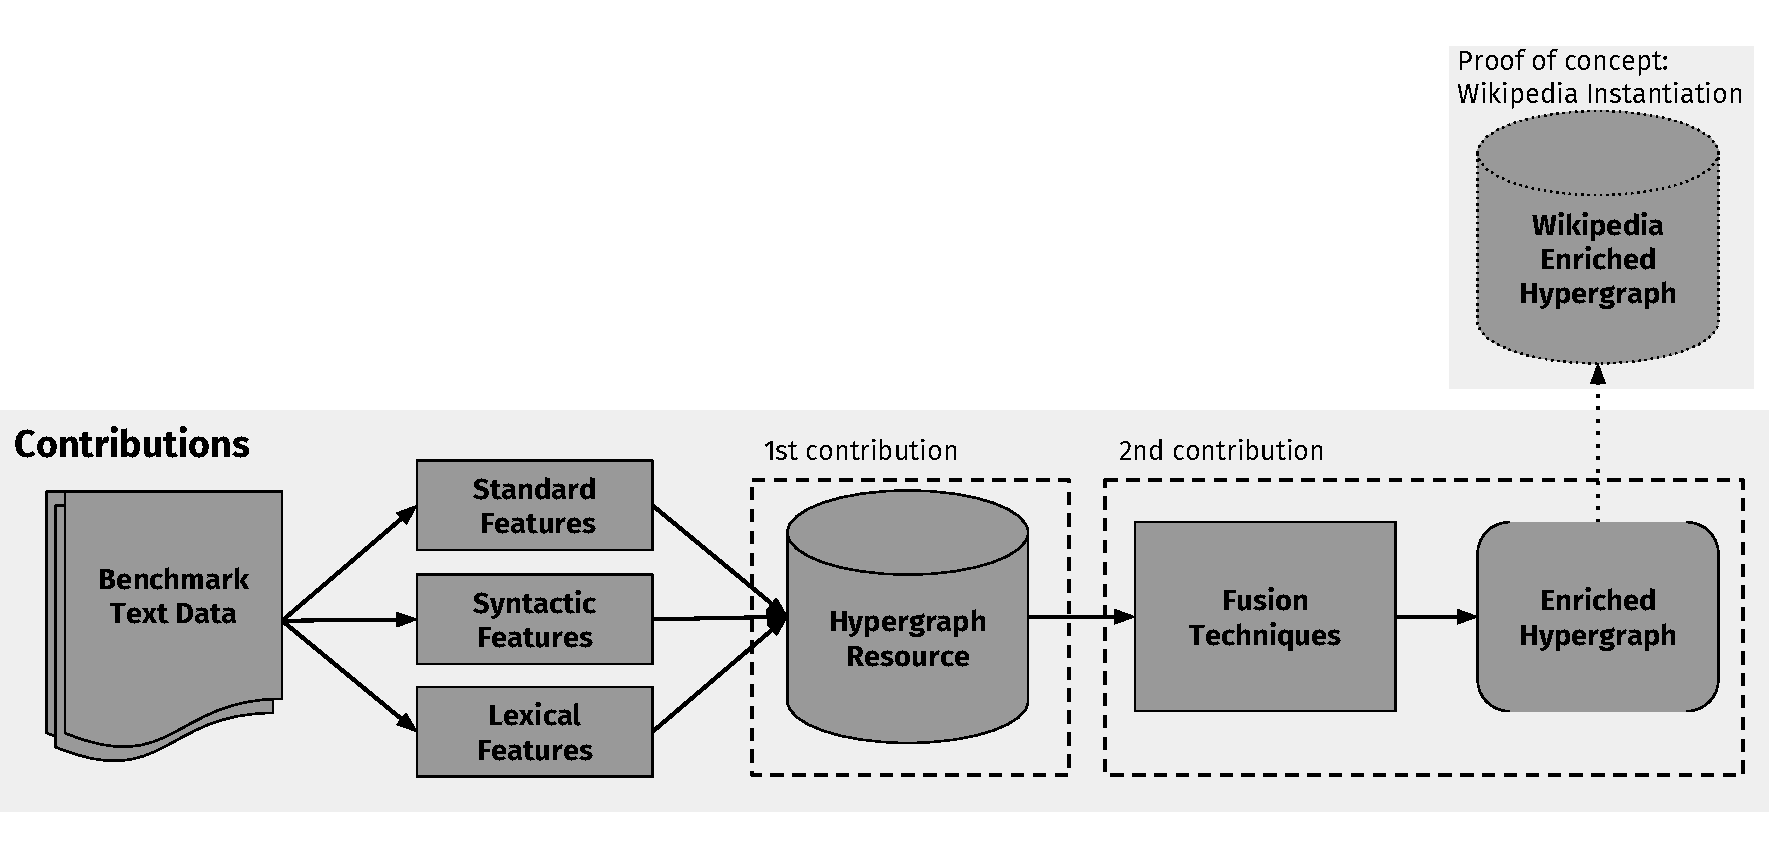
\includegraphics[width=1\linewidth]{./images/Chapitre3/main_diag_p1.pdf}
\caption{Modular description of the first two contributions of this work, described in this chapter. We see the elements of the fusion enriched hypergraph model we propose and its proof of concept instantiation.} 
%Also, at the bottom, the NLP tasks applications based on said model: word sense induction and disambiguation and named entity recognition.}
\label{fig:maindiag}
\end{figure}

In order to contextualize our proposition, we begin with the state of the art on how linguistic networks are employed in the literature. We are interested in those networks previously covered: lexical, syntactical and semantic co-occurrence networks. We give emphasis to two aspects: how the inner structure is used to solve the tasks at hand, and what type of graph-based algorithm is used. The literature on graph-based approaches for NLP is vast, we thus focus specifically on semantic tasks, notably Word Sense Induction and Disambiguation, and Named Entity Recognition. We chose these two tasks as we focus on both of them for the rest of our contributions. Afterwards, we introduce our model, how to build it  and its properties. We focus on the description of hypergraphs and how they allow us to join together different linguistic networks. Next, we introduce the concept of fusion techniques used to combine the linguistic features and obtain an enriched representation.

In that sense, this chapter presents a word representation model based on a generalization of graphs (we employ hypergraphs) that contains different types of linguistic data to characterize the terms (or words) contained within.  These representations are then combined with fusion techniques in order to ideally get an enriched and complementary feature space for each word. Finally, as a proof of concept, we describe the characteristics of the transformation of an English Wikipedia-based corpus into the framework we propose, a hypergraph model and its single enriched representation produced via fusion techniques. We show an example of the results produced by these fusion methods.

%The materialization of the proposed model allows us to computationally test the advantages as well as to discover the limitations of the proposed framework
%In the following chapter, we show in our experiments that this is indeed the case. 
.

\section{Linguistic Networks in Semantic NLP Tasks}\label{sec:ling_net_nlp}



We present here an overview of linguistic network's related work. We discuss what and how different methods are used with language networks to extract knowledge from their structural properties. Finally, we discuss the limitations of the current propositions and the advantages of the model we propose.
%\minitoc



\paragraph{Using Lexical Co-occurrence Networks}

Lexical Co-occurrence Networks (LCN) are  popular  since they do not require any special treatment to obtain them, just the input corpus. It is then natural that truly-unsupervised\footnote{Without the need of human-crafted semantic networks.} word sense induction approaches leverage these type of networks, and in return, the distributional hypothesis, to automatically discover senses for a given target word. That is why several WSI methods \cite{2004.Veronis,2007.Klapaftis.UOY,2010.Navigli.InducingWordSenses.Triangles,2008.Klapaftis.WSIUsingCollocations,2011.DiMarco.Navigli.ClusteringWebSearch,2011.Jurgens.WSICommunityDetection} are tightly related to LCNs. 
The cited works use a LCN as described before while other works such as \cite{2007.Navigli.GraphConnectivity,2014.Tao.Qian.LexicalChainHypergraphWSI} represent, as we do, the co-occurrence by means of a hypergraph scheme. In short, a hypergraph structure is a graph generalization where an edge (called hyperedge) can link more than two vertices per edge and thus it is able to provide a more complete description of the interaction between several nodes \cite{estrada2005}. In that sense, in  \cite{2014.Tao.Qian.LexicalChainHypergraphWSI} they make use of this type of representation to solve the task of word sense induction. Briefly, in this task we have to determine a set of senses for a given target word in a corpus, according to its context (a context here being usually a paragraph where the target word occurs). In their paper, given an input document with several context instances for each target word, they first extract lexical chains (set of semantically related words) from the contexts using a topic-modeling based technique. Secondly, a hypergraph is built where the vertices represent words and the hyperedges link two or more words if they exist in the same lexical chain. Thirdly, the hypergraph is clustered and groups of words are found which are considered to be the senses of the target word. Lastly, to assign these senses to each target word instance, they consider each sense as a vector, whose dimensions are each word in the corresponding cluster and its weight determines its level of co-occurrence  with the target word. The sense assignation is done by determining the similarity between sense vectors and a vectorial representation of each target word instance.

Generally, WSI systems generally perform four steps. Given an input text with a set of target words and their contexts (target words must have several instances throughout the document to cluster them), the steps are the following:

\begin{enumerate}
\item Build a LCN, assigning tokens as nodes and  establishing edges between them if they co-occur in a given context (usually if they both appear in the same sentence),
\item Determine the weights for each edge according to a frequency metric,
\item Apply a graph clustering algorithm. Each cluster found will represent a sense of the polysemous word, and
\item Match  target word instances with the clusters found by leveraging each target word context. Specifically, assign a cluster (a sense) to each instance by looking at the tokens in the context.
\end{enumerate}

As with semantic networks, not only WSD or WSI can be solved with LCNs. Finding semantic associated terms in a corpus is a critical step in several NLP systems. This task is solved in the system proposed by \cite{2011.Haishan.AHypergraphbased}. They also use a LCN although instead of a co-occurrence graph, they also employ a co-occurrence hypergraph, where nodes represent words and edges describe co-occurrence at the paragraph level.  In this work, they use such structure to find related terms in a given corpus. In order to do it, they mine the hypergraph as in a frequent itemsets problem, where the items are the words from a text. The method consists in first finding similar itemsets by means of measuring similarity between nodes. Once the 2-itemsets are found, they induce a graph from the original hypergraph by drawing edges between nodes that have a similarity superior to an arbitrary threshold. Lastly, in order to find $k$-itemsets ($k > 2$), the find either complete or connected components in the induced graph. 



As with WSD, while the LCNs used are mostly the same among approaches, there are certain moving parts that make up the difference between WSI approaches. The most common differences that can arise are:

\begin{itemize}
\item The clustering algorithm to find senses in the LCN graph.
\item The technique used to match context words to clusters.
\item The weight used in the graph edges.
\end{itemize}



\paragraph{Using Syntactic Co-occurrence Networks}

A network representation that is on the border line between being a LCN and a SCN is that of \cite{2013.Bronselaer.TextAnalysisWithGraphs}. They  propose a graph document modelization. In their network, nodes represent words and edges their co-occurrence, as any LCN. Still, their graph resembles a SCN because the edges may represent one of three types of words: either prepositions, conjunctions or verbs. As a result,  they need to first extract syntactic information from a document, namely the part-of-speech tags of each word. They find the most relevant words of a given text by ranking the nodes of the graph. The words that best represent a document can be used to summarize it, as they show in their work.

Approaches based on SCN are rarely used in WSD or WSI systems, and therefore they are an interesting research avenue to explore.




\paragraph{Using Semantic Networks}

Word sense induction is indeed a task usually solved using semantic networks, specially WordNet (and to a lesser extent, BabelNet) \cite{2004.Mihalcea.SemanticNetworkPageRank,2007.Sinha.Mihalcea.Unsupervised,2007.Tsatsaronis.WSDwithSpreading,2007.Navigli.GraphConnectivity,2008.Agirre.Multilingual,2008.Klapaftis.WSIUsingCollocations,2009.Agirre.PersonalizedPageRankWSD,2010.Klapaftis.WSD.WSD.HierarchicalGraphs,2010.Siberer.GraphCooccurrenceWSD,2014.Moro.Navigli.EntityLinking_WSD}. Given an input text with a set of ambiguous target words to process, these approaches follow a two-step algorithm:
\begin{enumerate}
\item Link target words (usually nouns, skipping stop-words and functional words) with their corresponding  sense (or synset in the case of WordNet-like dictionaries) and extract their vertices and edges into a new, smaller, SN. 
\item Apply a node ranking technique, usually a random-walk-based method, and select, for each ambiguous word in the input text,  its top ranking synset node as the correct sense.
\end{enumerate}

The amount of edges a SN has grows depending of the size of the version of WordNet used or the level of polysemy of a given word. In order to avoid redundancy or contradiction between  linking nodes, \cite{2004.Mihalcea.SemanticNetworkPageRank,2007.Navigli.GraphConnectivity} applied pruning techniques to avoid \textit{contamination} while calculating ranking metrics in order to define a pertinent sense. Regarding edge similarity measures,  in  \cite{2007.Sinha.Mihalcea.Unsupervised, 2007.Tsatsaronis.WSDwithSpreading} they test some metrics individually and also combined. They found that the best results are indeed obtained when several metrics are used at the same time.

%Other semantic tasks can also be solved using a SN. For example, Entity linking \cite{2014.Moro.Navigli.EntityLinking_WSD}. In their work, they leverage the BabelNet LKB to jointly disambiguate and link polysemous words to Wikipedia articles. 

Concerning the measure of semantic affinity between two terms, in \cite{2009.Yeh.Wikiwalk} they quantify word similarity by means of projecting them into a Wikipedia space. First, they represent each word by a vector representing its most pertinent pages,  and then they calculate a vectorial similarity measure between them.

%In \cite{2013.Matuschek.Gurevych.Dijsktra.WSA} they propose a technique that aligns SNs, i.e., they link senses from two different networks. This task is called word sense alignment. Several SNs are used (WordNet, Wikipedia, Wiktionary, etc.) thus nodes can represent synsets, articles, or concepts. The links may depict semantic relations or may be links joining two concepts or pages together. Their approach aims to find the shortest path between nodes of any two given SNs while leveraging already existing links between  equal concepts found in both SNs.



Finally, extracting entities from text can also benefit from the use of SNs. The work proposed by  \cite{2013.Kivimaki.AGraph-BasedApproach} aims to extract technical skills from a document. Again, using Wikipedia as SN, they first represent each article and the input document in a token vector space model.  Next, they find the document top 200 similar pages by calculating the cosine similarity between the document and each page. This serves to extract a Wikipedia subgraph which is used to calculate the most relevant pages for the entry document. Finally, the top pages are filtered by means of selecting those articles that actually represent a skill using a fixed list of skill-related tokens. Once again, the nodes represent Wikipedia articles and the edges the hyperlinks that join them.


The cited methods vary in how they make use of their SN, not so much in the network per se. These differences boil down to three aspects:
\begin{bulletList}
\item Type of relationship implied by the edges linking the nodes of the network, 
\item The algorithm used to rank the nodes after the semantic network is built, and
\item The weight assigned to each edge.
\end{bulletList}

\paragraph{Using Heterogeneous Networks}

Even though this kind of structure seems to open new avenues of research in the semantic analysis domain, only few explicitly take advantage of them, as is the case of \cite{2013.Saluja.Graph-BasedUnsupervisedLearning}. In their approach, they build a graph that links together features with words, and discover similarity measures that leverage the multi-typed nature of their network.


\subsection{Algorithms used in Linguistic Networks}

We have discussed until now the different types of networks from a content point of view. In this subsection, we address the details of the graph-based algorithms used to solve semantic NLP tasks. In this section we cover the details of four different types of graph algorithms.

%\paragraph{Notation}
%In this section we will be referring to a connected undirected graph, which we denote by $G = (V,E,W)$. The graph $G$ has vertex set $V$, edge set $E$ where $|V|=n$, $|E|=m$, and the matrix $W\in\mathbb{R}^{n\times n}$, with $w_{u,v} \geq 0$, defines any kind of weights in the graph.


\paragraph{Edge Weights}

We begin by describing the metrics used to determine similarity between nodes, usually stored as edge weights. As stated in the previous sections, most of the metrics are frequency based, specially when dealing with LCNs. The main idea of these measures is to assign a weight that decreases as the association frequency of the words increases. Among these measures, the most popular are the Dice  coefficient \cite{2010.Navigli.InducingWordSenses.Triangles,2011.DiMarco.Navigli.ClusteringWebSearch,2013.DiMarco.Navigli.ClusteringGraph-BasedWSI}, normalized pointwise mutual information \cite{2013.Hope.GradedWSI}, and a graph-adapted tf-idf variant \cite{2007.Tsatsaronis.WSDwithSpreading} which aims to give importance to frequent edges while also favoring those that are rare.

Edge weights can also be calculated when the vertices of a network do not represent words. Such is the case of \cite{2010.Klapaftis.WSD.WSD.HierarchicalGraphs}, where nodes represents a target word context (set of tokens around an ambiguous word). This time the Jaccard index is used to quantify similarity between them while considering how many words are shared between a pair of context nodes.

When the nodes represent synsets (or concepts), certain approaches leverage only the intrinsic nature of the network connections, leveraged by random walk algorithms, without explicitly using  weighted edges \cite{2004.Mihalcea.SemanticNetworkPageRank}. 
 On the other hand, there are techniques that assign a frequency-based weight to represent the importance of a semantic relation, particularly those found in the reviews  by \cite{2007.Sinha.Mihalcea.Unsupervised,2007.Navigli.GraphConnectivity}, where several weights are tested.

A  more sophisticated approach to edge weighting is proposed in \cite{2013.Saluja.Graph-BasedUnsupervisedLearning} where they employ  custom-defined functions in order to learn the most appropriate edges' weights for a given set of seed vertices inside a network. The main idea  is to enforce \textit{smoothness} (keeping two nodes close if they have related edges) across the network.

As a way to rank edges according to their importance, the ratio of triangles (cycles of length 3), squares (cycles of length 4), and diamonds (graphs with 4 vertices and 5 edges, forming a square with a diagonal) in which an edge participates are calculated \cite{2010.Navigli.InducingWordSenses.Triangles,2013.DiMarco.Navigli.ClusteringGraph-BasedWSI}. Once the top edges are found, they create a subgraph containing only these edges (and its corresponding vertices).

Finally, instead of applying weights to edges, a case where  nodes are weighted can be found in \cite{2013.Kivimaki.AGraph-BasedApproach}. They measure and remove popular nodes in order to avoid their bias during the application of their random walk approach.




 

\paragraph{Graph Search}
Usually, in a WSD approach, the first step to follow is to build a graph from a LKB. The goal is to explore the semantic network and find all the senses linked to  those found in the context of an ambiguous word. Aside from custom search heuristics applied by certain works \cite{2006.Agirre.TwoGraph-basedAlgorithms,2007.Sinha.Mihalcea.Unsupervised,2009.Agirre.PersonalizedPageRankWSD}, researchers also use well-known graph techniques such as depth-first search \cite{2007.Navigli.GraphConnectivity}, breadth-first search \cite{2008.Agirre.Multilingual} and even the Dijsktra  algorithm to find the group of closest senses in the network \cite{2013.Matuschek.Gurevych.Dijsktra.WSA}.


\paragraph{Node Connectivity Measures}\label{sec:connectivity_measures}
A Connectivity Measure (CM) determines the importance of a node in a graph according to its association with other nodes. In most cases its value ranges from zero to one, where the 0 indicates that the node is of minor importance while 1 suggests a relatively high significance. Nowadays, the most widely used  measures are those based on random walks.

A Random Walk (RW) can be simply defined as the traversal of a graph beginning from a given node and randomly jumping to another in the next time step.
% It is similar to a Markov chain process, the difference being that in a Markov chain the next step node is chosen to according to a certain distribution.  

PageRank \cite{Brin1998}, the popular random walk based algorithm is used commonly in WSD. The recursive intuition of PageRank is to give importance to a node according to the PageRank value of the nodes that are connected to it. %Formally, the vector PageRank holding values for each node in $v \in V$ is calculated as: $PR(v) = \alpha\sum_{u,v\in E}{\frac{PR(u)}{outdegree(u}} + \mathbf{v}(1-\alpha)$, where $ \alpha  $ is a dumping factor to control the jumps a random walker will make; and $ \mathbf{v} $ is the relevance vector for each node has in $G$. In classical PageRank, the values of  $\mathbf{v}$ are uniformly set to $\frac{1}{n}$ for all nodes in $|V|$. 
Nonetheless, as a regular random-walk algorithm, in PageRank the probability distribution to change from a node to another is uniform. In such case, the jumps a random walker performs depend solely on the nature of the graph studied. Among the approaches surveyed, those that use the most PageRank are those that solve word sense disambiguation \cite{2004.Mihalcea.SemanticNetworkPageRank,2006.Agirre.TwoGraph-basedAlgorithms,2007.Navigli.GraphConnectivity,2010.Siberer.GraphCooccurrenceWSD}. 
%
These approaches make a conventional use of PageRank: they apply it and rank nodes to select the most appropriate senses for ambiguous words. Still, there are some improvements over the classical use of PageRank in WSD. Some techniques employ a different version of PageRank called Personalized PageRank (or PageRank with restart \cite{Murphy2012} or PPR) were a random walker may return to a specific starting node with certain probability rather than jumping to a random node. This formulation allows researchers to assign more weight to certain nodes. For example, in \cite{2009.Agirre.PersonalizedPageRankWSD} they are able to use the complete Wordnet graph as their SN. They do this by directly adding context words of a polysemous token into Wordnet and then giving a uniform initial distribution to only these nodes. In this way, they force PageRank to give more importance to the context words without the need of extracting a subgraph from the SN. In \cite{2014.Moro.Navigli.EntityLinking_WSD} they apply the same technique to obtain a \textit{semantic signature} of a given sense vertex. After applying PPR, they obtain a frequency distribution over all the  nodes in the graph. The so-called semantic signature consists in those nodes that were visited more than an arbitrary threshold and that best represent an input sense node.

There are other methods which share the properties of random walk approaches. In  \cite{2007.Tsatsaronis.WSDwithSpreading,2013.Kivimaki.AGraph-BasedApproach} they apply a method known as spreading activation. This algorithm aims to iteratively diffuse the initial weights of a set of seed nodes across the network. Specifically, once a weighted semantic network is built, they \textit{activate}  the nodes representing the context senses, assigning a value of 1, while \textit{deactivating} the rest by setting them to 0. They determine the most pertinent senses to the input nodes by storing, for each of them, the last active sense node with the highest activation value. 

Beyond WSD and into the task of determining word similarities, we found the work of \cite{2009.Yeh.Wikiwalk}, where they calculate a semantic similarity between a pair of words while leveraging a Wikipedia SN. For each word, they  apply PPR to find the articles that best represent a word. 
%They set the initial distribution in such a way that the articles that best represent each word have a higher probability than the rest of nodes. 
In \cite{2013.Saluja.Graph-BasedUnsupervisedLearning}, they also employ PPR to find synonym words given a word-similarity matrix and a new unknown word (also known as out-of-vocabulary word). They link the new word to its corresponding feature nodes and they normalize the similarity matrix to use the weights as probabilities and thus bias the random walk. In \cite{2013.Kivimaki.AGraph-BasedApproach} they use centrality measures to determine the most relevant nodes in a SN and then, in contrast with most approaches, remove them from the graph in order to not bias their graph algorithms.
%

With regard to other CMs, there are  more elementary alternatives to determine the importance of a node. For example, the approaches of  \cite{2004.Veronis,2007.Klapaftis.UOY,2011.Haishan.AHypergraphbased,2013.Bronselaer.TextAnalysisWithGraphs,2014.Moro.Navigli.EntityLinking_WSD} successfully use the degree of a node, or other metric, to determine its importance in a network.






\paragraph{Graph Clustering/Partitioning}

Graph clustering is defined as the task of grouping the vertices of a graph into clusters while taking into consideration its edge structure \cite{Schaeffer2007}. As previously mentioned, graph-based word sense induction relies most importantly in the graph clustering step where the actual senses of a word are inferred. 

In this subsection we also consider  subgraph extracting techniques which are exploited to find separated groups of words and thus induce senses. In this context we found the approaches of \cite{2004.Veronis,2010.Siberer.GraphCooccurrenceWSD}. These systems make use of both the Minimum and Maximum Spanning Trees algorithms (MinST and MaxST, respectively) as a final step to  disambiguate a target word given its context.  Meanwhile, both \cite{2011.Haishan.AHypergraphbased,2014.Tao.Qian.LexicalChainHypergraphWSI}  use the Hypergraph Normalized Cut (HCT) approach, a hypergraph clustering method based on minimum cuts, to induce senses.

Most of the reviewed approaches employ state of the art techniques \cite{2008.Klapaftis.WSIUsingCollocations,2010.Klapaftis.WSD.WSD.HierarchicalGraphs,2011.Jurgens.WSICommunityDetection,2013.Hope.GradedWSI}. Specifically, they utilize Chinese Whispers (CW) \cite{biemann2006chinese}, Hierarchical Random Graphs (HRG) \cite{clauset2008hierarchical}, Link Clustering (LC) \cite{ahn2010link}, and MaxMax (MM) \cite{hope2013maxmax} respectively. 

Briefly, CW is a randomized graph-clustering method  which is time-linear with respect to the number of edges and does not need a fixed number of clusters as input. It only requires a maximum amount of iterations to perform. HRG, being a hierarchical clustering algorithm, groups words into a binary tree representation, which allows to have more in-detail information about the similarity among words when compared to flat clustering algorithms. Regarding LC, instead of clustering nodes, this procedure groups edges. Thus it can identify contexts related to certain senses, instead of finding groups of words as most approaches do. Finally, MM, is able to assemble words into a fixed cluster (hard clustering) or allow them to be in several groups at the same time (soft clustering). It shares certain characteristics with CW:  they are both methods that exploit similarity within the local neighborhood of nodes and both are time-linear. Nonetheless, a key difference is that CW is not deterministic, while MM is, thus MM will find always the same clustering result for the same input graph.

 
 


\begin{table}[]
\centering
\caption{Survey summary table.}
\label{tab:survey_sum}
\setlength\tabcolsep{1.8mm}
\def\arraystretch{.95}%
\begin{tabular}{l|cccc|cccc}
\hline
\textbf{\textbf{Approach}}                                                       & \multicolumn{4}{c|}{\textbf{Network Type}}                                                                                                              & \multicolumn{4}{c}{\textbf{Algorithms}}                                                                                                                                                                                                                            \\ \hline
                                                                                 & \rotatebox[origin=c]{90}{Semantic} & \rotatebox[origin=c]{90}{Lexical} & \rotatebox[origin=c]{90}{Syntactic} & \rotatebox[origin=c]{90}{Heterogeneous} & \rotatebox[origin=c]{90}{Edge Wts.} & \rotatebox[origin=c]{90}{Graph Search} & \rotatebox[origin=c]{90}{Connectivity Meas.} & \rotatebox[origin=c]{90}{Graph Clust.} \\ \hline
Veronis, 2004 \cite{2004.Veronis}                                                &                                    & x                                 &                                     &                                         &                                                                                  &                                        & x                                               & x                                                                                    \\
Mihalcea et al., 2004 \cite{2004.Mihalcea.SemanticNetworkPageRank}               & x                                  &                                   &                                     &                                         &                                                                                  &                                        & x                                               &                                                                                      \\
Agirre et al., 2006 \cite{2006.Agirre.TwoGraph-basedAlgorithms}                  &                                    & x                                 &                                     &                                         &                                                                                  & x                                      & x                                               &                                                                                      \\
Sinha and Mihalcea, 2007 \cite{2007.Sinha.Mihalcea.Unsupervised}                 & x                                  &                                   &                                     &                                         &                                                                                  & x                                      &                                                 &                                                                                      \\
Navigli and Lapata, 2007\cite{2007.Navigli.GraphConnectivity}                    & x                                  &                                   &                                     &                                         &                                                                                  & x                                      & x                                               &                                                                                      \\
Tsatsaronis et al., 2007 \cite{2007.Tsatsaronis.WSDwithSpreading}                & x                                  &                                   &                                     &                                         &                                                                                  &                                        & x                                               &                                                                                      \\
Klapaftis and Manandhar, 2007 \cite{2007.Klapaftis.UoY}                          &                                    & x                                 &                                     &                                         & x                                                                                &                                        & x                                               &                                                                                      \\
Klapaftis and Manandhar, 2008 \cite{2008.Klapaftis.WSIUsingCollocations}         &                                    & x                                 &                                     &                                         & x                                                                                &                                        &                                                 & x                                                                                    \\
Agirre and Soroa, 2008 \cite{2008.Agirre.Multilingual}                           & x                                  &                                   &                                     &                                         &                                                                                  & x                                      &                                                 &                                                                                      \\
Agirre and Soroa, 2009 \cite{2009.Agirre.PersonalizedPageRankWSD}                & x                                  &                                   &                                     &                                         &                                                                                  & x                                      & x                                               &                                                                                      \\
Klapaftis and Manandhar, 2010 \cite{2010.Klapaftis.WSD.WSD.HierarchicalGraphs}   &                                    & x                                 &                                     &                                         & x                                                                                &                                        &                                                 & x                                                                                    \\
Navigli and Crisafulli, 2010 \cite{2010.Navigli.InducingWordSenses.Triangles}    &                                    & x                                 &                                     &                                         & x                                                                                &                                        &                                                 &                                                                                      \\
Silberer and Ponzetto, 2010 \cite{2010.Siberer.GraphCooccurrenceWSD}             &                                    & x                                 &                                     &                                         &                                                                                  &                                        & x                                               & x                                                                                    \\
Di Marco and Navigli, 2011 \cite{2011.DiMarco.Navigli.ClusteringWebSearch}       &                                    & x                                 &                                     &                                         & x                                                                                &                                        &                                                 &                                                                                      \\
Jurgens, 2011 \cite{2011.Jurgens.WSICommunityDetection}                          &                                    &                                   &                                     &                                         &                                                                                  &                                        &                                                 & x                                                                                    \\
Di Marco and Navigli, 2013 \cite{2013.DiMarco.Navigli.ClusteringGraph-BasedWSI}  &                                    & x                                 &                                     &                                         & x                                                                                &                                        &                                                 &                                                                                      \\
Hope and Keller, 2013 \cite{2013.Hope.GradedWSI}                                 &                                    &                                   & x                                   &                                         & x                                                                                &                                        &                                                 & x                                                                                    \\
Moro et al., 2014 \cite{2014.Moro.Navigli.EntityLinking_WSD}                     & x                                  &                                   &                                     &                                         &                                                                                  &                                        & x                                               &                                                                                      \\
Qian et al., 2014 \cite{2014.Tao.Qian.LexicalChainHypergraphWSI}                 & x                                  & x                                 &                                     &                                         &                                                                                  &                                        &                                                 & x                                                                                    \\
Yeh et al., 2009 \cite{2009.Yeh.Wikiwalk}                                        & x                                  &                                   &                                     &                                         &                                                                                  &                                        & x                                               &                                                                                      \\
Liu et al., 2011 \cite{2011.Haishan.AHypergraphbased}                            &                                    & x                                 &                                     &                                         &                                                                                  &                                        & x                                               & x                                                                                    \\
Matuschek and Gurevych, 2013 \cite{2013.Matuschek.Gurevych.Dijsktra.WSA}         & x                                  &                                   &                                     &                                         &                                                                                  & x                                      &                                                 &                                                                                      \\
Bronselaer and Pasi, 2013  \cite{2013.Bronselaer.TextAnalysisWithGraphs}         &                                    &                                   & x                                   &                                         &                                                                                  &                                        & x                                               &                                                                                      \\
Kivim\"{a}ki et al., 2013 \cite{2013.Kivimaki.AGraph-BasedApproach}              & x                                  &                                   &                                     &                                         & x                                                                                &                                        & x                                               &                                                                                      \\
Saluja and Navr\'{a}til, 2013 \cite{2013.Saluja.Graph-BasedUnsupervisedLearning} &                                    & x                                 &                                     & x                                       & x                                                                                &                                        & x                                               &                                                                                      \\ \hline
\multicolumn{1}{c}{25}                                                           & 11                                 & 12                                & 2                                   & 1                                       & 9                                                                                & 6                                      & 14                                              & 8                                                                                    \\ \hline
\end{tabular}
\end{table}


\subsection{Discussion}\label{sec:disc_chap3}
We have covered the network attributes of several approaches on semantic related NLP tasks. A summary of these strategies is shown in Table \ref{tab:survey_sum}.
In this section we shortly discuss the reviewed articles from a  modelization perspective as well as looking at the evolution of the approaches used to solve the word sense disambiguation and induction tasks.


Regarding WSD approaches, we see that the use of a lexical knowledge base, such as Wordnet, is pervasive in this task. Indeed, new resources, such as BabelNet, solves to some extent the fixed (no new senses are included automatically) nature of this type of resources by leveraging the always evolving knowledge of Wikipedia. Indeed, in the recent years, entity linking has emerged as a related task to WSD. It takes even more advantage from bases that combine both Wordnet and Wikipedia, such as BabelNet. On the other hand, WSI, while being a more flexible approach (language and word-usage independent, does not require human-made bases)  for solving WSD, its results are tightly linked to the quality of the clustering algorithm used. 
% 
%We refer to  linguistic-network modelization as the type of linguistic information and the means in which it is stored within a language network.
 With respect to the networks' modelization, we find that few approaches deal with syntactic attributes. We believe that finding semantic similarities can be improved by adding syntactic information not only  while using dependency relations but also by leveraging the constituency tree of each word. Moreover, using syntactic data along with semantic and/or lexical co-occurrences takes us into the heterogeneous network domain which has not been addressed in most of the approaches covered. Being able to design new similarity metrics that deal with different types of information opens new avenues of research in the semantic similarity domain. Finally, concerning the algorithms employed, few approaches make direct use of the graph Laplacian representation. New similarities could be defined using the Laplacian as a starting point. 


Taking into account the described opportunities of research, in the following section we propose a  hypergraph modelization of a linguistic network that aims to solve some limitations stated above. 


 
\section{Proposed Model: Fusion Enriched Hypergraph Linguistic Network}
\label{sec:enriched_hypergraph}

As stated before, our model consists on two parts (and two contributions). The first one, an hypergraph model that holds different types of linguistic relations extracted from a corpus. And the second one, the combination of linguistic features in order to generate a less sparse, enriched representation. 

In this section we focus on the first part, the hypergraph model. We note that for the sake of simplicity we limit ourselves to lexical and syntactic information. The model in essence holds two different networks, one for each type of relations. They are both unified by means of a hypergraph structure. 

\subsection{Hypergraph Linguistic Model}

 Formally, a hypergraph \cite{Berge1985} is a graph generalization  that allows more than two vertices to be linked by a single edge.  We call $\mathcal{H}=(V,E)$ a {hypergraph}
 with the {vertex} set $V$ and the hyperedge set $E$. Let $V$ denote a finite set of objects, and let $E$  (the hyperarcs or hyperedges) be a
group of subsets  of $V$ such that $V = \cup_{e_j \in E}e_j$.
%todo add biblio how hypergraphs are used in NLP??
A \emph{weighted hypergraph} is a hypergraph that has a positive number $w(e)$ associated with each hyperedge, called the \emph{weight} of the hyperedge $e$. A \emph{weighted hypergraph} is then denoted by $\mathcal{H}=(V,E,w)$.
%
A hyperedge $e$ is said to be \emph{incident} with a vertex $v$ when
$v \in e$.
 As one can see, as in regular graph theory, the adjacency is referred to the elements of the same kind (vertices vs vertices, or edges vs edges), while the incidence is referred to the elements of different kind (vertices vs edges).

\begin{figure}
\centering
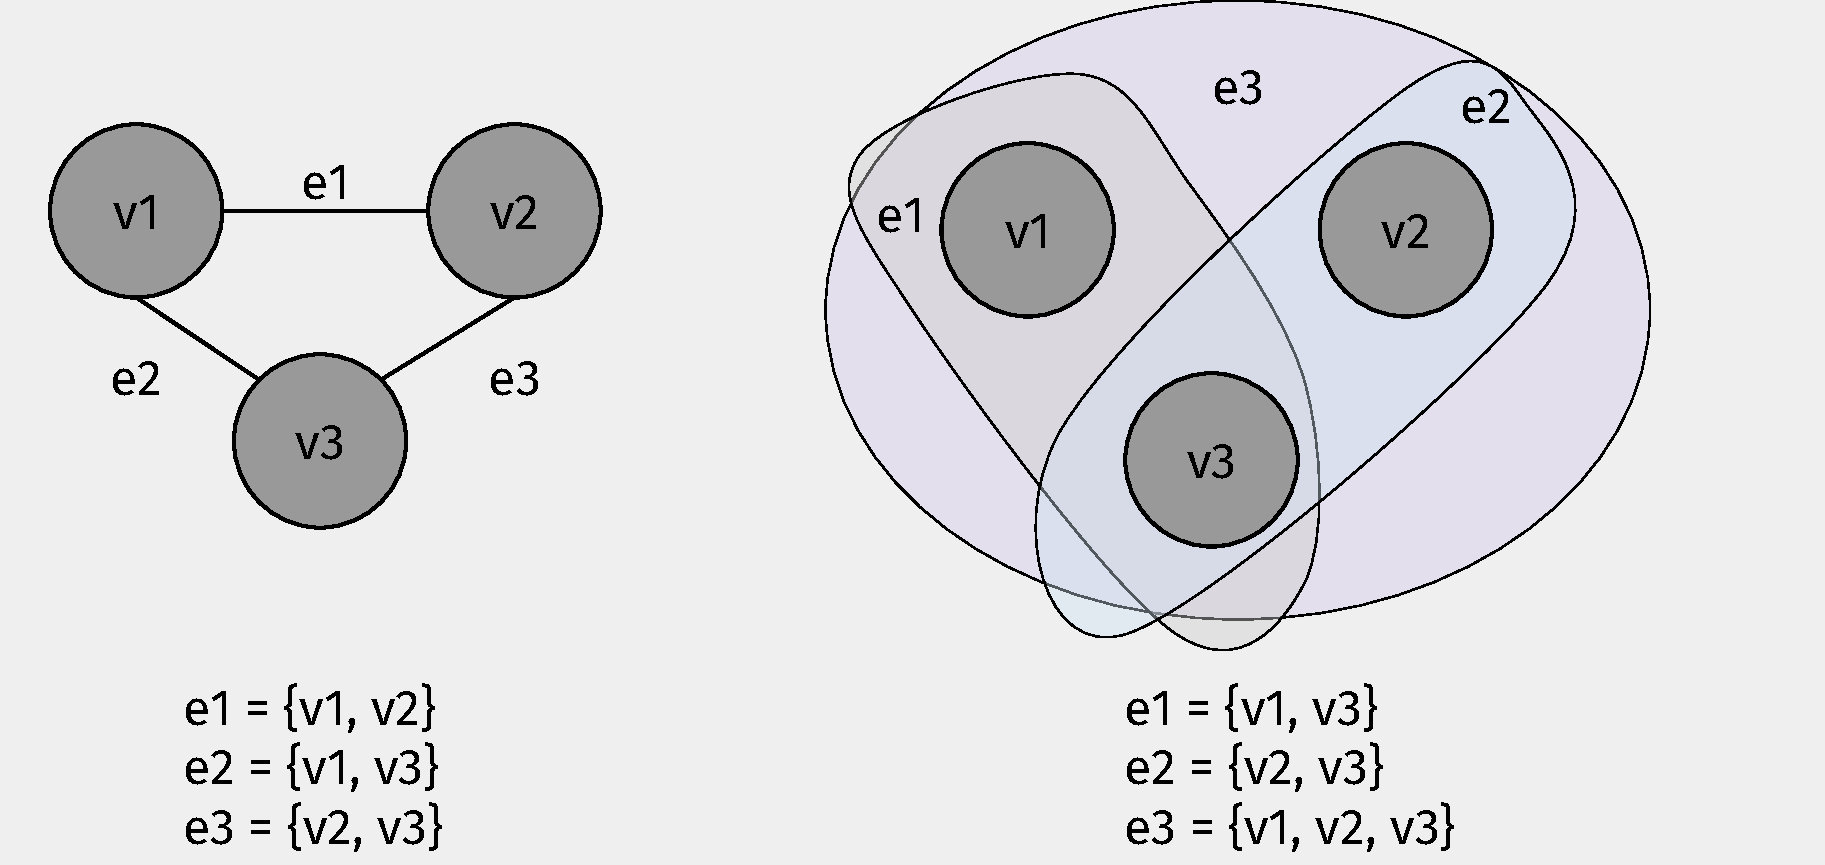
\includegraphics[width=0.7\linewidth]{images/Chapitre3/graph_vs_hgraph.pdf}
\caption{A graph (to the left) compared to a hypergraph (to the right). The edges of the hypergraph (hyperedges) may hold more than two nodes at once, relaxing the constraint of graphs' binary relations. A hypergraph can be seen as a set of $n$-ary sets: $E=\{\{v1,v3\},\{v2,v3\},\{v1,v2,v3\}\}$.}
\label{fig:graph_vs_hgraph}
\end{figure}


Building upon previous linguistic representations \cite{2007.Klapaftis.UOY,2011.Haishan.AHypergraphbased,2014.Tao.Qian.LexicalChainHypergraphWSI}, our model is indeed based on the use of a hypergraph.
% As stated before, hypergraphs have been employed in the literature to model complex systems. 
Their single most important difference with regular graphs, being able to relate more than two vertices at the same type, allows for a better characterization of interactions within a set of individual elements (in our case, words) \cite{heintz2014beyond}. Indeed, our hypergraph modelization initially integrates four types of relations between tokens: sentence co-occurrence, part-of-speech tags, words' constituents data and dependency relations in a single linguistic structure. These relationships were chosen because it is relatively easy to obtain them for high-resource languages. These features can be seen as building blocks for NLP models. Extracting deeper language features would implicate relying even more on general domain systems. In any case, our goal is to arrive to more complex annotations (e.g., named entities) from the selected features and relations. Indeed, as we discussed before, different types of contexts gives us different types of similarities. Recall that a  smaller lexical window  gives us co-occurrence relations that approach functional relatedness, such as those found with syntactic contexts. That is why we decided to keep a lexical context at sentence level, so that it may complement the distributional semantic information provided by the dependency functions context as well as the phrase-constituency syntactic context. In short, we  aim to cover three levels of possible semantic relatedness via  three levels (in terms of the size of the neighborhood of a target word) of distributional co-occurrences 
%todo (see Figure \ref{})
: a short range with dependency functions, a medium range with phrase constituency membership, and a longer range with sentence lexical co-occurrences. The intuition is that when solving NLP tasks, having direct access to these three semantic spaces will help to determine a more appropriate meaning's relation between words. 

 
\paragraph{Construction}
In our case, the set of words in the corpus are the set of nodes  $V$, and the set of hyperedges  $E$ represent the relations between nodes according to different linguistic aspects.
%
We consider each word (i.e., each node) to exist in one of three types of hyperedges, two syntactic and one lexical co-occurrence contexts:
\begin{enumerate}
\item $\textsc{\textbf{NP}}$: noun phrase (NP)  constituents,
\item $\textsc{\textbf{DEP}}$: dependency relations. We consider all types of dependency functions between nouns and verbs,
\item  $\textsc{\textbf{SEN}}$: lexical context, in this case the window considered is the whole sentence
\end{enumerate} 

The part of speech information is stored implicitly with the constituent information. While these parameters are fixed in our implementation, they can easily be adapted to other configurations. For example, we may consider noun phrases and verb phrases as chunks, specific types of dependency functions, or different lexical window size.

To populate the hypergraph, given a token $v$, a noun phrase $p$, a sentence $s$, and a 
dependency function $dep(h, \cdot)$, with $h$ being the head of the relation, we consider the following rules:

\begin{itemize}
\item $v$ is incident (or belongs) to a hyperedge $e_j$ of type $\textsc{\textbf{NP}}$ if  $v$ appears in the same noun phrase $p$.
\item The same condition is used with sentence hyperedges $\textsc{\textbf{SEN}}$: if  $v$ appears in a sentence $s$, it will be located in a hyperedge $e_j$ of type $\textsc{\textbf{SEN}}$. 
\item If $v$ participates in a dependency function $dep(h,v)$ as a dependent, it belongs to a hyperedge $e_j$ of type $\textsc{\textbf{DEP}}$.
\end{itemize}

Each hyperedge is labeled according to an identifier that allows the hypergraph to be populated while reading words from a corpus. For example, the hyperedges of the set $\textsc{\textbf{SEN}}=\{h_{S_1}, h_{S_2}, h_{S_3}\}$ are indeed hyperedges that represent sentences, identified by an index in this case. Hyperedges $h_{S_1}, h_{S_2}, h_{S_3}$ contain each a set of words. Additionally, the hypergraph can be represented as a $n \times m$ incidence $H$ matrix with entries $h(i,j) = N(v_i, e_j)$ where $N(v_i, e_j)$ is the number of times $v_i \in e_j$ occurs in the corpus. This frequency values can be later converted into other weighting schemes as seen in Chapter \ref{chap:backgnd}. Indeed, the incidence matrix allows us to pass from the hypergraph-based model of representation into the vector-space model.

\paragraph{Running Example}
We illustrate the process of creating a sample hypergraph model with the following example phrase: \textit{The report contains copies of the minutes of these meetings}.  We tokenize the phrase, keeping all the words, and we lemmatize and parse it to obtain both constituency and dependency trees. 

\subparagraph{Constituency Tree} The constituency tree of the example phrase is shown in Figure \ref{fig:tree_constits}. The sentence, as well as each noun phrase (\textit{NP}) node is identified by a number, these numbers serve as an unique identifier of the phrase chunk within the whole sentence. We can observe that this phrase is composed by five noun phrases and one verb phrase. Meanwhile, some \textit{NP} are formed by other kind of phrases, depending on the grammar production rule used to build each one of them. Furthermore, as is usual in this kind of structures, there is a one to one relation between the number of tokens in the sentence  and the number of leaves in the tree.

For clarity,  in our example we  only consider nouns and the first three noun phrases (from left to right), as well as the nominal subject (\textit{nsubj}) and direct object (\textit{dobj}) dependency relations. Thus, in total, as described below, we have three hyperedges of noun phrase type: $NP_1, NP_2$ and $NP_3$. Each of them corresponding to the noun phrases in the constituents tree.
 
\subparagraph{Dependency Tree}
The dependencies of the example phrase are shown in Figure \ref{fig:tree_deps_report} as a tree structure. The relations can also be seen as tuples in Table \ref{tab:depends_report} In these relations' examples, the head is the first token to appear  followed by the dependent word. Two hyperedges are found: 
$nsubj_{contains}$ and $dobj_{contains}$.
 \begin{figure}
 \centering
 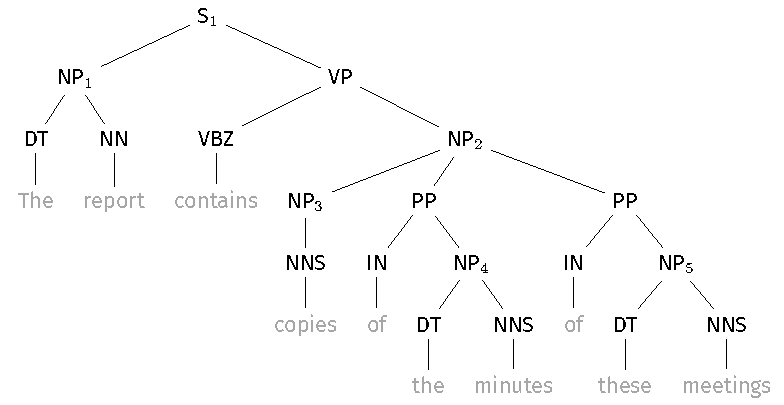
\includegraphics[width=0.7\linewidth]{images/Chapitre3/trees/tree_constits.pdf}
 \caption{Constituency-based tree of the phrase \textit{The report contains copies of the minutes of these meetings.}}
 \label{fig:tree_constits}
 \end{figure}
 
 %todo compare levels of semanticity in the three proposed models
 %
 
\begin{figure}[]
	\begin{minipage}{\textwidth}
		\begin{minipage}{.9\textwidth}
		\centering
		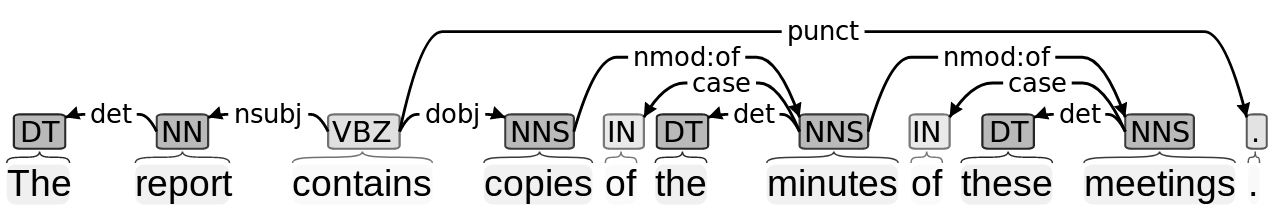
\includegraphics[width=0.9\linewidth]{images/Chapitre3/tree_deps_report.png}
		\captionof{figure}{Dependency-based tree of the example phrase.}
		\label{fig:tree_deps_report}
		\end{minipage} 
		\vspace{1cm}
		
		\begin{minipage}{.9\textwidth}
		\centering
		\begin{tabular}{@{}ll@{}}
%		 \toprule
		 \textbf{root}(root, contains)    & \textbf{det}(minutes, the)       \\
		 \textbf{det}(report, The)        & \textbf{nmod:of}(copies, minutes)   \\
		 \textbf{dobj}(contains, copies)  & \textbf{det}(meetings, these)    \\
		 \textbf{nmod:of}(minutes, meetings)       & \textbf{nmod}(minutes, meetings) \\
		 \textbf{nsubj}(contains, report) &
		 \end{tabular}
		 \captionof{table}{Dependency relations of the example phrase.}
		 \label{tab:depends_report}
		\end{minipage} 
	\end{minipage}	
\end{figure}


 
\subparagraph{Hyperedges Found}
From both syntactic parses and the phrase itself we build a hypergraph representation as stated before.  We show below the hyperedges sets found for each type,  ($\textsc{\textbf{NP}}$, $\textsc{\textbf{SEN}}$, and $\textsc{\textbf{DEP}}$), and their members. Each hyperedge  is labeled  with a unique identifier:
%todo imagen con el hypergrafo completo would be nice
\begin{itemize}
\item $\textsc{\textbf{NP}}=\{NP_1, NP_2, NP_3\}$
	\begin{itemize}
		\item $NP_1=\{report\}$	
		\item $NP_2=\{copies,\,minutes,\,meetings\}$
		\item $NP_3=\{minutes\}$
	\end{itemize}
\item $\textsc{\textbf{SEN}}=\{S_1\}$
	\begin{itemize}
		\item $S_1=\{report,\,contains,\,copies,\,minutes,\,meetings\}$	
	\end{itemize}
\item $\textsc{\textbf{DEP}}=\{nsubj_{contains},\,dobj_{contains}\}$
	\begin{itemize}
		\item $nsubj_{contains}=\{report\}$	
		\item $dobj_{contains}=\{copies\}$	
	\end{itemize}

\end{itemize}

\subparagraph{Incidence Matrix}We can represent these hyperedges as an incidence matrix, illustrated in Figure \ref{fig:incidence_report}.  
Looking at the table, we can   infer that the word \textit{copies} appears  in two hyperedges of type $\textsc{\textbf{NP}}$: first in \textit{NP$_2$}, which is built from a noun phrase  and two prepositional phrases (\textit{PP}). Secondly, we see that it is part of \textit{NP$_3$}, which  indicates a plural noun (\textit{NNS}).
Regarding the syntactic dependency hyperedges, the word \textit{copies} appear in the \textit{dobj} \textit{contains} column which indicates that \textit{copies} was the direct object of the verb \textit{contains}. Concerning the sentence hyperedges, we see that the token \textit{copies} appeared in the same sentence S$_1$ as the other four noun words.

\begin{figure}
\centering
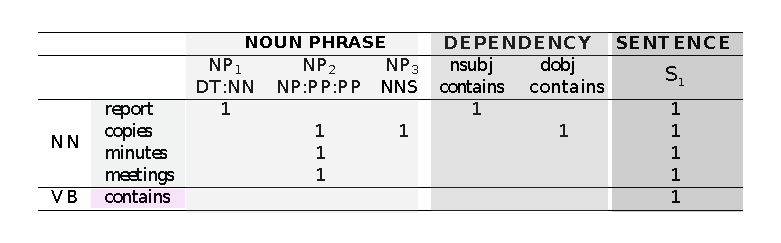
\includegraphics[width=\linewidth]{images/Chapitre3/incidence_mat.pdf}
\caption{Incidence matrix of the example phrase hypergraph modelization.}
\label{fig:incidence_report}
%todo change font to fira of this pic!
\end{figure}


%\paragraph{Discussion}
With the short example we show the intuitive way in which we identify three different kinds of relations: lexical co-occurrence (at sentence level), dependency co-occurrence, and noun phrase co-occurrence. Looking at the incidence matrix we see the three levels of semantic relatedness we aim to represent with the three different types of context: sentence, dependency, and noun phrase level. At the same time, there is a structure within the hypergraphs. Groups of words are found to be together either directly or by means of paths traced by other nodes. 

On the other hand, we realize that it is sparse\footnote{Sparse for the  size of this example incidence matrix. Sparsity increases as more text is included in the hypergraph.}. Sparsity, as we saw previously, affects the performance of knowledge discovery techniques applied to NLP tasks. 

Just as the literature approaches covered before, we aim to solve semantic tasks by using the proposed linguistic resource and its relations. Yet, unlike those approaches we have three contexts and thus three levels of semantic relatedness, coupled to the $n$-ary relations from the hypergraph structure. Nonetheless, our model also suffers from data sparsity. We will show how to deal with this issue in the following section. The general idea is that by combining features from the different contexts we can alleviate the problem as similarities not seen in a context may complement the features from another context. The set of approaches that perform this combination are known as multimedia fusion techniques.
% We can thus build systems that allow us to interpret a word from different perspectives according to said relations.




                                                                                            
\subsection{Representation Enrichment with Fusion Techniques}\label{sec:fusion}
 
%We first describe below multimedia (or multimodal) fusion techniques  as well as relevant use cases where they have been employed. 
%Then, we focus exclusively on fusion techniques applied to NLP tasks, which is the general domain of the two tasks (NER and WSI/WSD) we focus on.                   
The second part of our proposed method deals with the fusion of textual features. Namely, we combine the features that describe terms into a single representation space. This new space aims to address two issue that arise while working with textual data: effectively using information coming from different linguistic levels (e.g., lexical, syntactic, semantic) while alleviating the sparsity typical of textual representations.

Multimodal fusion is a set of popular techniques used in multimedia analysis tasks. These methods integrate multiple media features, the affinities among these attributes or the decisions obtained from systems trained with said features, to obtain rich insights about the data being used and thus to solve a given analysis  task \cite{AtreyHEK10}. We note that these techniques come at the price of augmenting the complexity of a given system by increasing or reducing the sparsity of a given feature matrix.


In the multimodal fusion literature we can discern two main common types of techniques: early fusion and late fusion. A third and fourth type of fusion methods, cross-media fusion and hybrid fusion are also employed in multimedia analysis tasks. 

These four fusion operators naturally address the issue of dealing with heterogeneous data as they all mix one way or another the feature columns from each of two representations. Regarding alleviating sparsity, the intuition is that by combining matrices either by element-wise summing or multiplying them, the resulting matrix will have a denser structure. For example, by summing two matrices with the same shape, such as two term-term similarity matrices, we  obtain a resulting matrix that contains the similarities of both feature spaces. In the same sense , when multiplying two matrices we combine them while also obtaining a denser output matrix. Nonetheless, both sum and multiplication result depends evidently on the nature of the matrices employed. Two of the fusion techniques mentioned above, late fusion and cross-media fusion use sum and multiplication as they  main matrix operator. What is more, both of them contemplate the use of similarity matrices as at least one of their inputs. Being similarity matrices, they tend to be dense and thus the resulting sum or product will be more dense than the original sparse representation, while complementing and enriching the space with other types of information. We present an example of this intuition in the following section.


We describe the four of them in the following paragraphs. The notation used is first introduced as follows: the fusion functions are binary, they all take two inputs, parameters $A$ and parameter $B$ which define arbitrary single-modality matrices. For example, both matrices $A$ and $B$ may represent a lexical $M^{L}$, syntactical based $M^{S}$, or other type representation spaces $M^{T}$. On the other hand, they may also describe their  respective similarity (square) matrices, $S^{L}$ and  $S^{S}$. In a broader sense, matrices $A$ and $B$ may represent any pair of valid\footnote{Valid in terms of having compatible shapes while computing a matrix sum or multiplication.} term-feature matrices.



\paragraph{Early Fusion}
This technique is the most widely used fusion method. The principle is simple: we take both modal features and concatenate them into a single representation matrix. More formally, we consider two matrices  that represent different modality features each  over the same set of individuals. To perform early fusion we concatenate them column-wise, such that we form a new matrix having the same number of lines but increasing the number of columns to the sum of the number of columns of both matrices. The matrices may also be weighted as to control the influence of each modality.

Such trivial fusion  is shown in Figure \ref{fig:ef_diag}. In this example, two  matrices are used, $\mlex$ and $\msyn$. They both have the same number of rows $n$, they have $m$ and $p$ columns, respectively. After an early fusion operation, the final matrix  has $m+p$ features. Formally, the early fusion function is defined as:
\begin{equation}
E(A,B) = \mathbf{hstack}(A , B)
\end{equation}
As stated before, the matrices $A$ and $B$ are combined together via a concatenation function $\mathbf{hstack}$ which joins both of them column-wise. In order for this operator to work, both matrices must have the same $n$ number of rows.

During the concatenation, we may also apply a weight to matrices $A$ and $B$ such as: 
\begin{equation}
E_\alpha(A,B) = \mathbf{hstack}(\alpha\cdot A , (1-\alpha)\cdot B)
\end{equation}
Indeed, this weighted early fusion  represents the same operation as before with an extra parameter: $\alpha$, which controls the relative importance of each matrix. In the following, we refer to both operations simply as early fusion. When $\alpha$ is determined (and indicated as a subscript), we refer to weighted early fusion. Otherwise, there is no weighting scheme applied to the operation.

The main advantage of early fusion is that a single unique model is fitted while leveraging the correlations among the concatenated features. The method is also easy to integrate into an analysis system. The main drawback is that we increase the representation space and may make it harder to fit models over it.

\begin{figure}
\centering
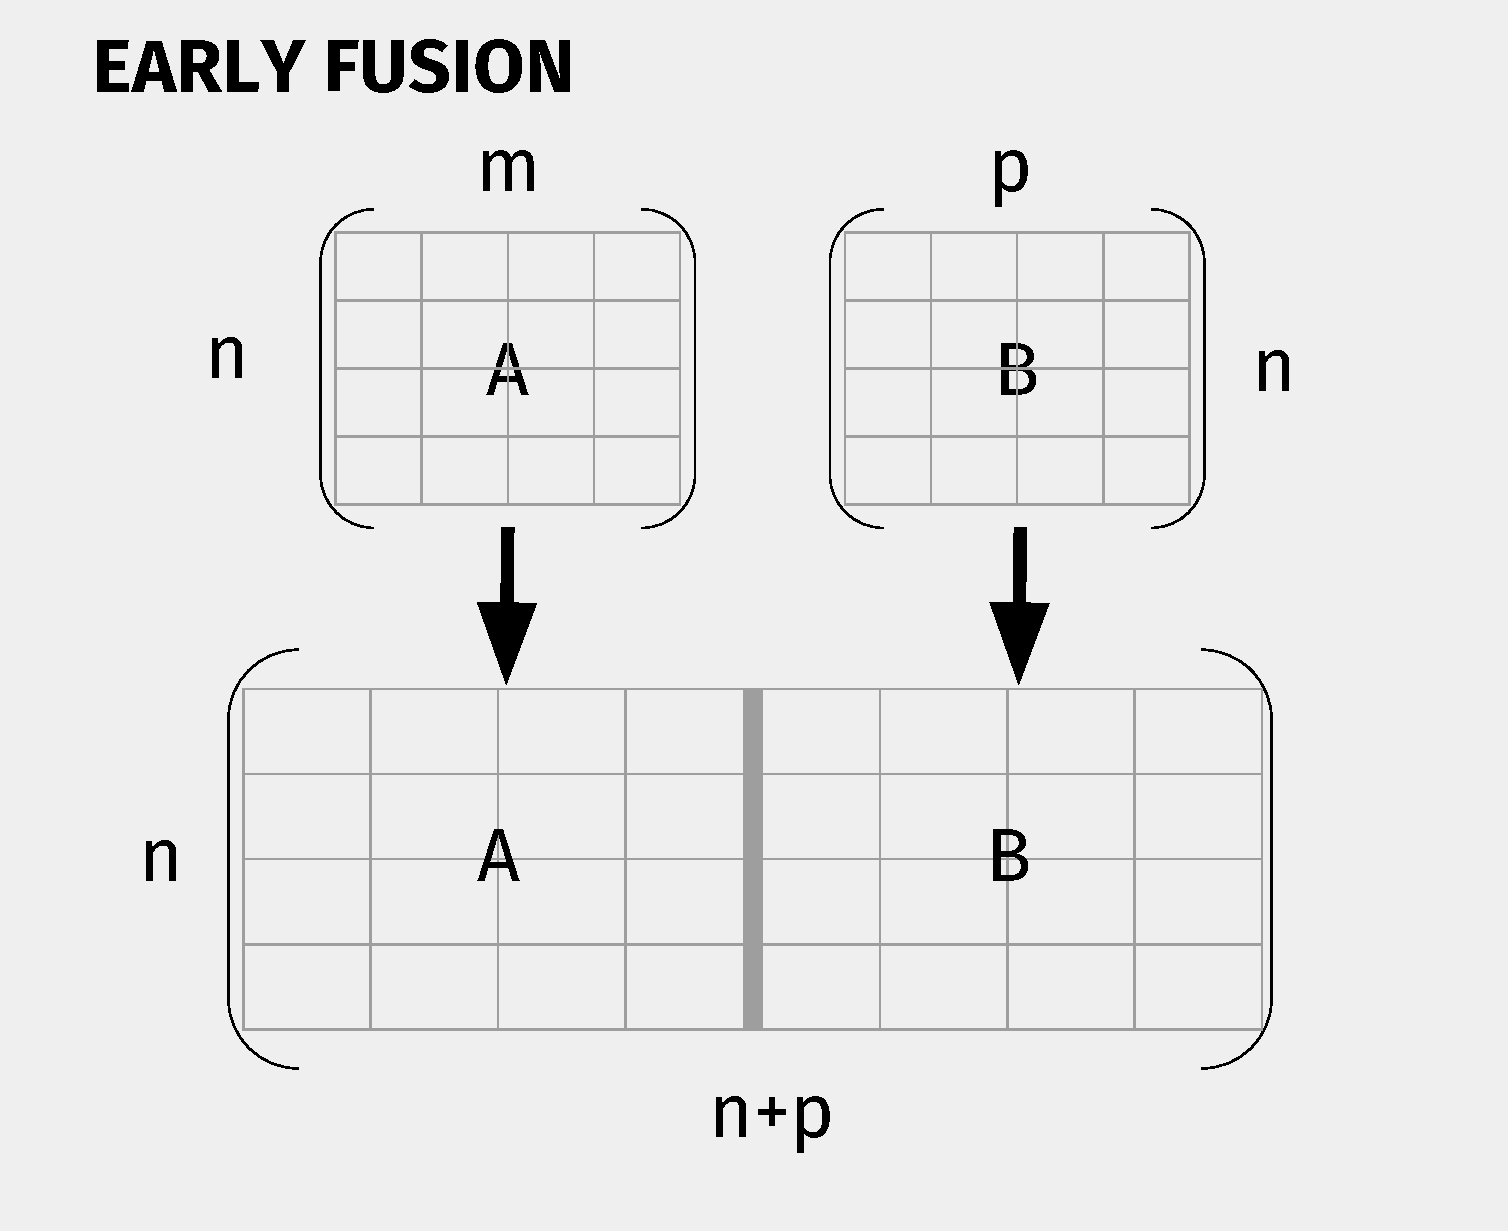
\includegraphics[width=0.7\linewidth]{images/Chapitre3/ef_diag.pdf}
\caption{Early Fusion of feature matrices $A$ and $B$. The result is the concatenation of both matrices.}
\label{fig:ef_diag}
\end{figure}


%

%   of shape $(n, m + p)$. Following the literature notation of [vulic], the early fusion representation matrix EF is defined as:
%\begin{equation}
%EF = \alpha \times X_1 || (1 - \alpha) \times X_2
%\end{equation}

%where $||$ represents the column-wise concatenation operation and ? is the parameter that determines the contribution of each modality. 
%
%Early fusion has been employed in several multimodal tasks. For example, [?]. 
\paragraph{Late Fusion}
In contrast to early fusion, in late fusion the combination of multimodal features are generally performed at the decision level, i.e., using the output of independent knowledge discovery models trained  each with a unique set of features \cite{ClinchantAC11}. In this setting,  decisions produced by each model are combined into a single final result set. The diagram in Figure \ref{fig:lf1} shows this combination of matrices $A$ and $B$.
%
The methods used to combine preliminary decisions usually involve one of two types: rule-based (where modalities are combined according to domain-specific knowledge) or linear fusion (e.g., weighting and then adding or multiplying both matrices together). This particular type of fusion is very close to machine learning  ensemble methods.
%

Indeed, late fusion combines both modalities in the same semantic space. In that sense,  we may also combine modalities via an affinity representation instead of final decision sets. In other words, we may combine two modalities  by means of their respective similarity matrices. In this case, a  representation is  obtained by adding  two similarity matrices, as in Figure \ref{fig:lf2}. In the figure, we use the equal-sized matrices $A\prime$ and $B\prime$, which in this case are the similarity matrices of inputs $A$ and $B$. Both matrices are then summed to produce a single $n \times n$ weighted matrix (determined by a parameter $\beta$). 
%

More formally, we define the late fusion function as:
\begin{equation} \label{eq:late-fusion}
L_\beta(A,B) = \beta \cdot A + (1 - \beta)\cdot B
\end{equation}

In this function, the extra parameter $\beta$ affects the influence of matrix $A$,  and consequently also the relevance of matrix $B$. As we are summing two matrices, for this operator both $A$ and $B$ must be of the same size.


The advantages of late fusion include the combination of features at the same level of representation (either the fusion of decisions or similarity matrices). Also, given that independent models are trained separately, we can choose which algorithm is more adequate for each type of features. 



\begin{figure}
	\centering
	\begin{subfigure}[t]{.5\textwidth}
	\centering
	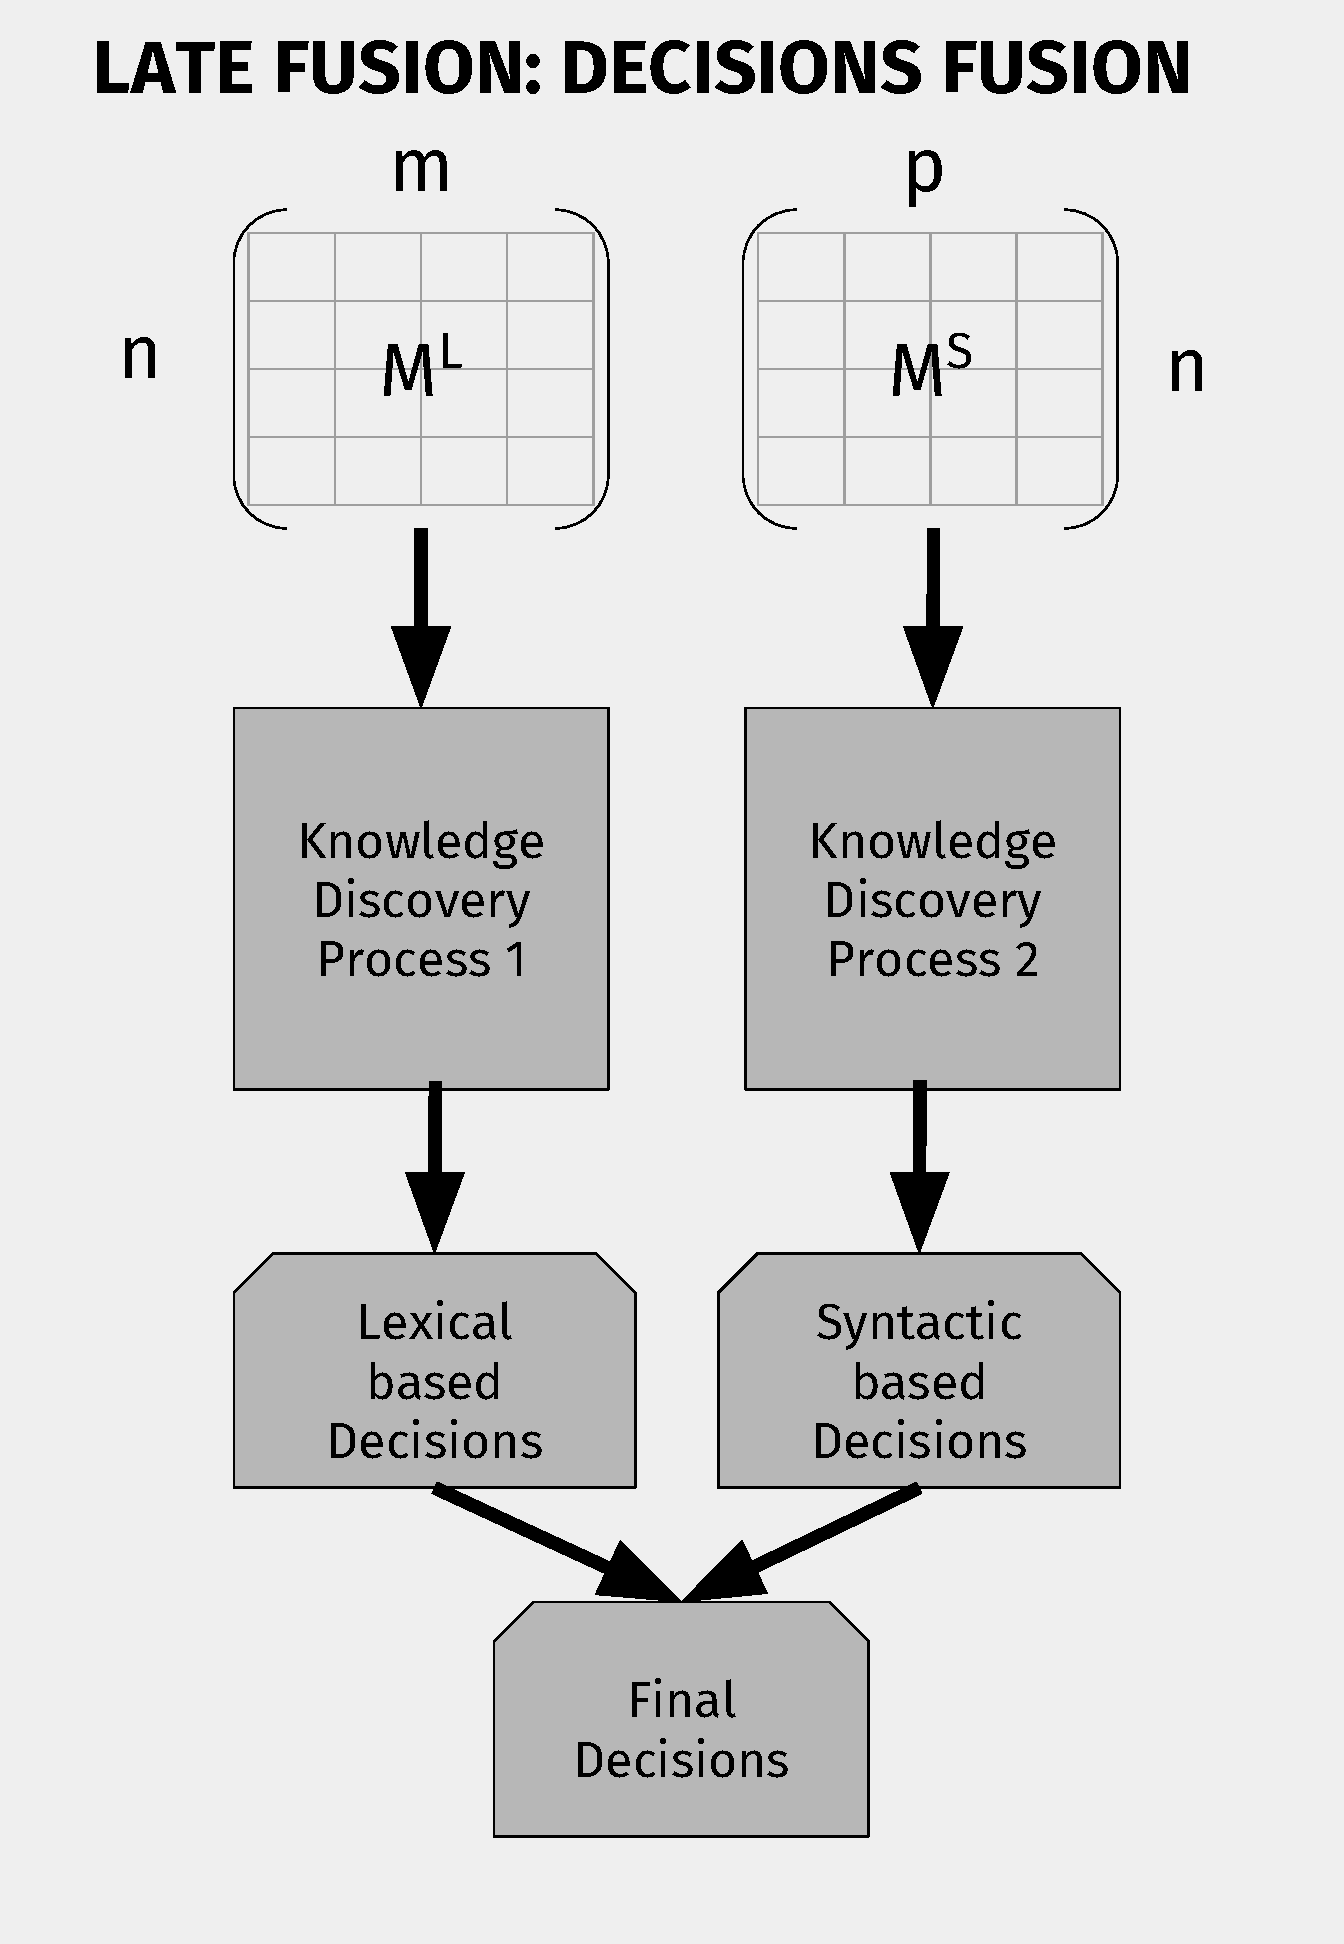
\includegraphics[width=0.9\linewidth]{images/Chapitre3/lf1_diag.pdf}
	\caption{Fusion of decisions.}
	\label{fig:lf1}
	\end{subfigure}% 
	\begin{subfigure}[t]{.5\textwidth}
	\centering
	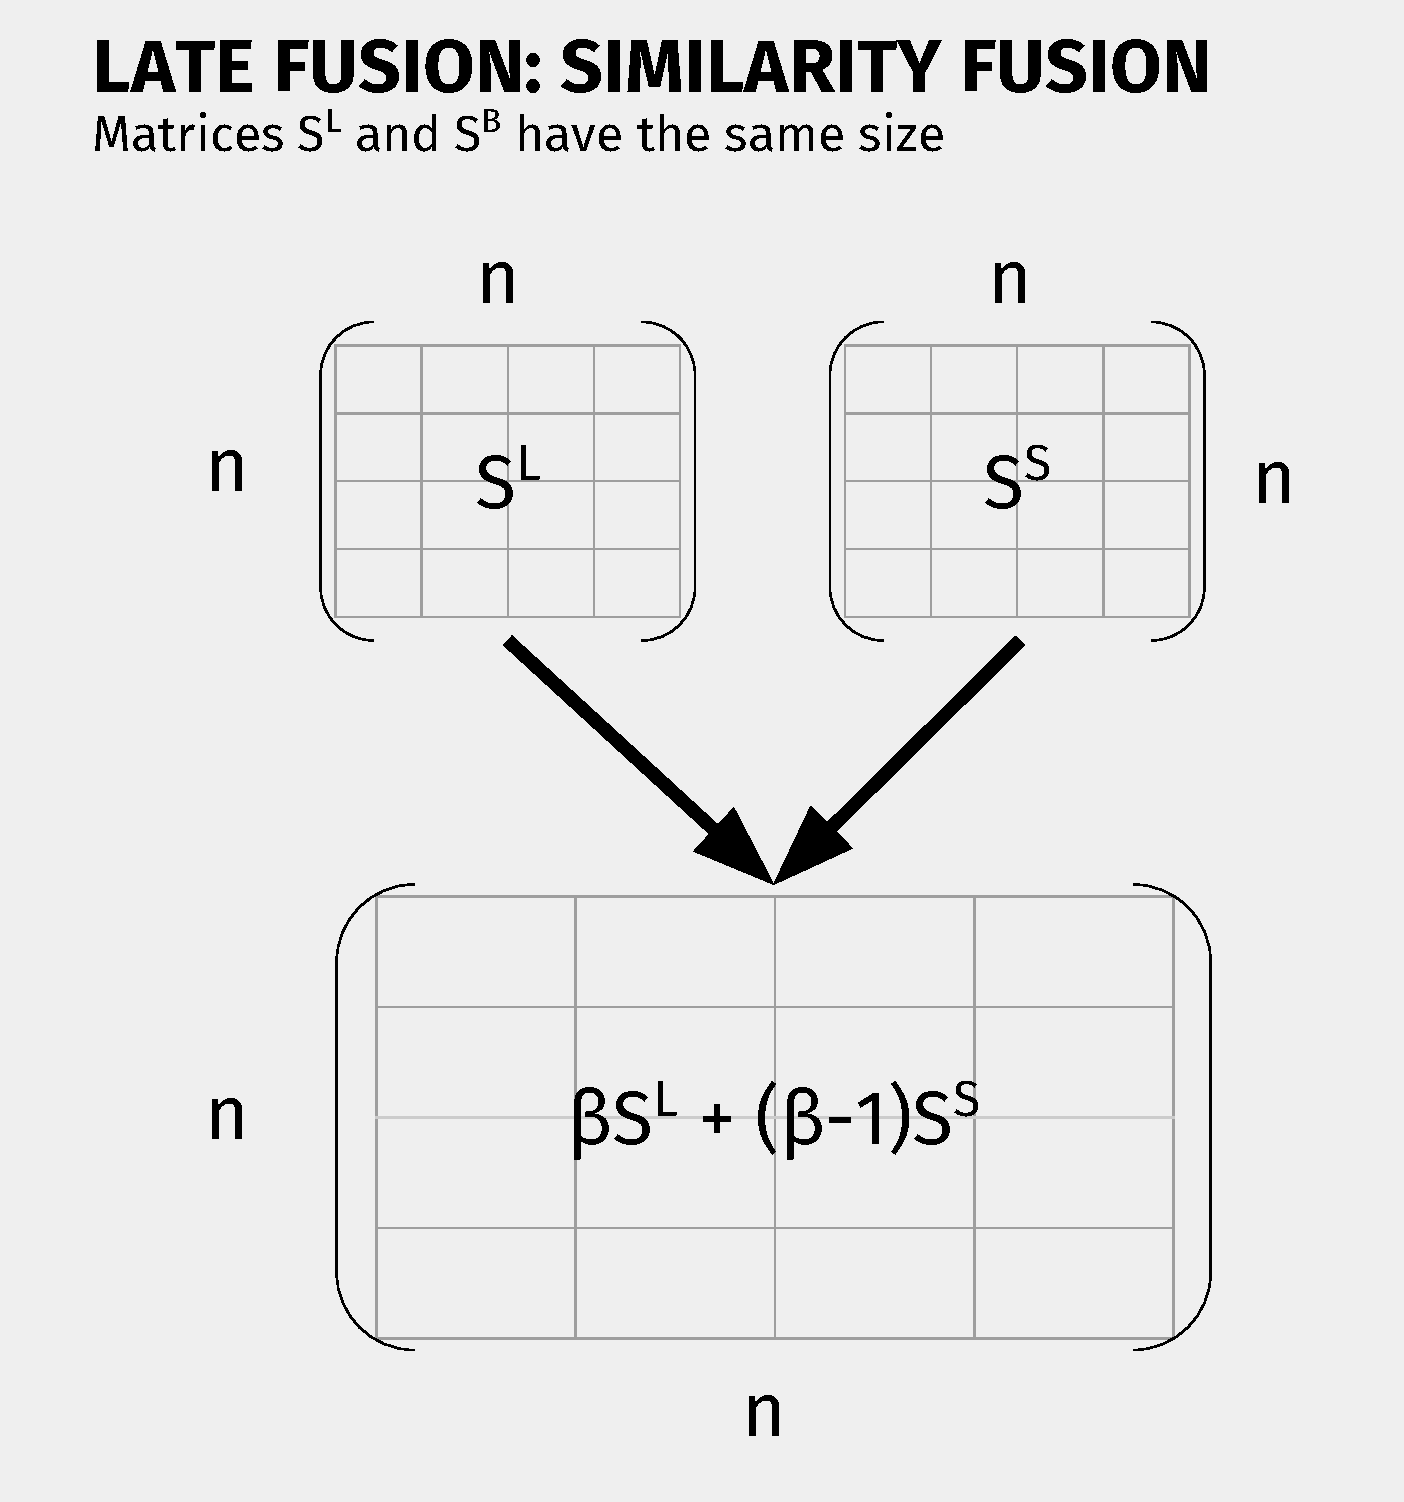
\includegraphics[width=0.9\linewidth]{images/Chapitre3/lf2_diag.pdf}
	\caption{Fusion of similarity matrices.}
	\label{fig:lf2}	
	\end{subfigure}
	\caption{Late fusion possibilities. To the left, fusion of knowledge discovery models' decisions. To the right, fusion of similarity matrices.}
	\label{fig:lf_diag}
\end{figure}




%For example, in information retrieval (Ah-Pine et al., 2015), lexicon learning (Vulic et al., 2016), coreference resolution (Eisenstein and Davis, 2007); different types of representations (different modalities) can be combined in order to take advantage of the complementarity existing among them
\paragraph{Cross-media  Fusion}
%
A third type of fusion technique, cross-media  fusion (or simply cross fusion),   introduced in \cite{ClinchantAC11,Ah-PineCC15}, is defined and employed to propagate a single similarity matrix into a second similarity matrix. In their paper, the authors propagated information from textual media towards visual media. In our case, we transfer information among textual features. For example, to perform a cross fusion between lexical and syntactical features, we perform the following steps: 
\begin{enumerate}
\item Compute the corresponding similarity matrices for each type of features.
\item Keep only the $k$-nearest neighbors for each word within the lexical similarity matrix while assigning zero to the rest.  These selected neighbors are to be used as lexical representatives to enrich the syntactical similarities.
\item Linearly combine both similarity matrices (lexical $k$-nearest lexical neighbors with the syntactical features) via a matrix product.
\end{enumerate}  

\begin{figure}
\centering
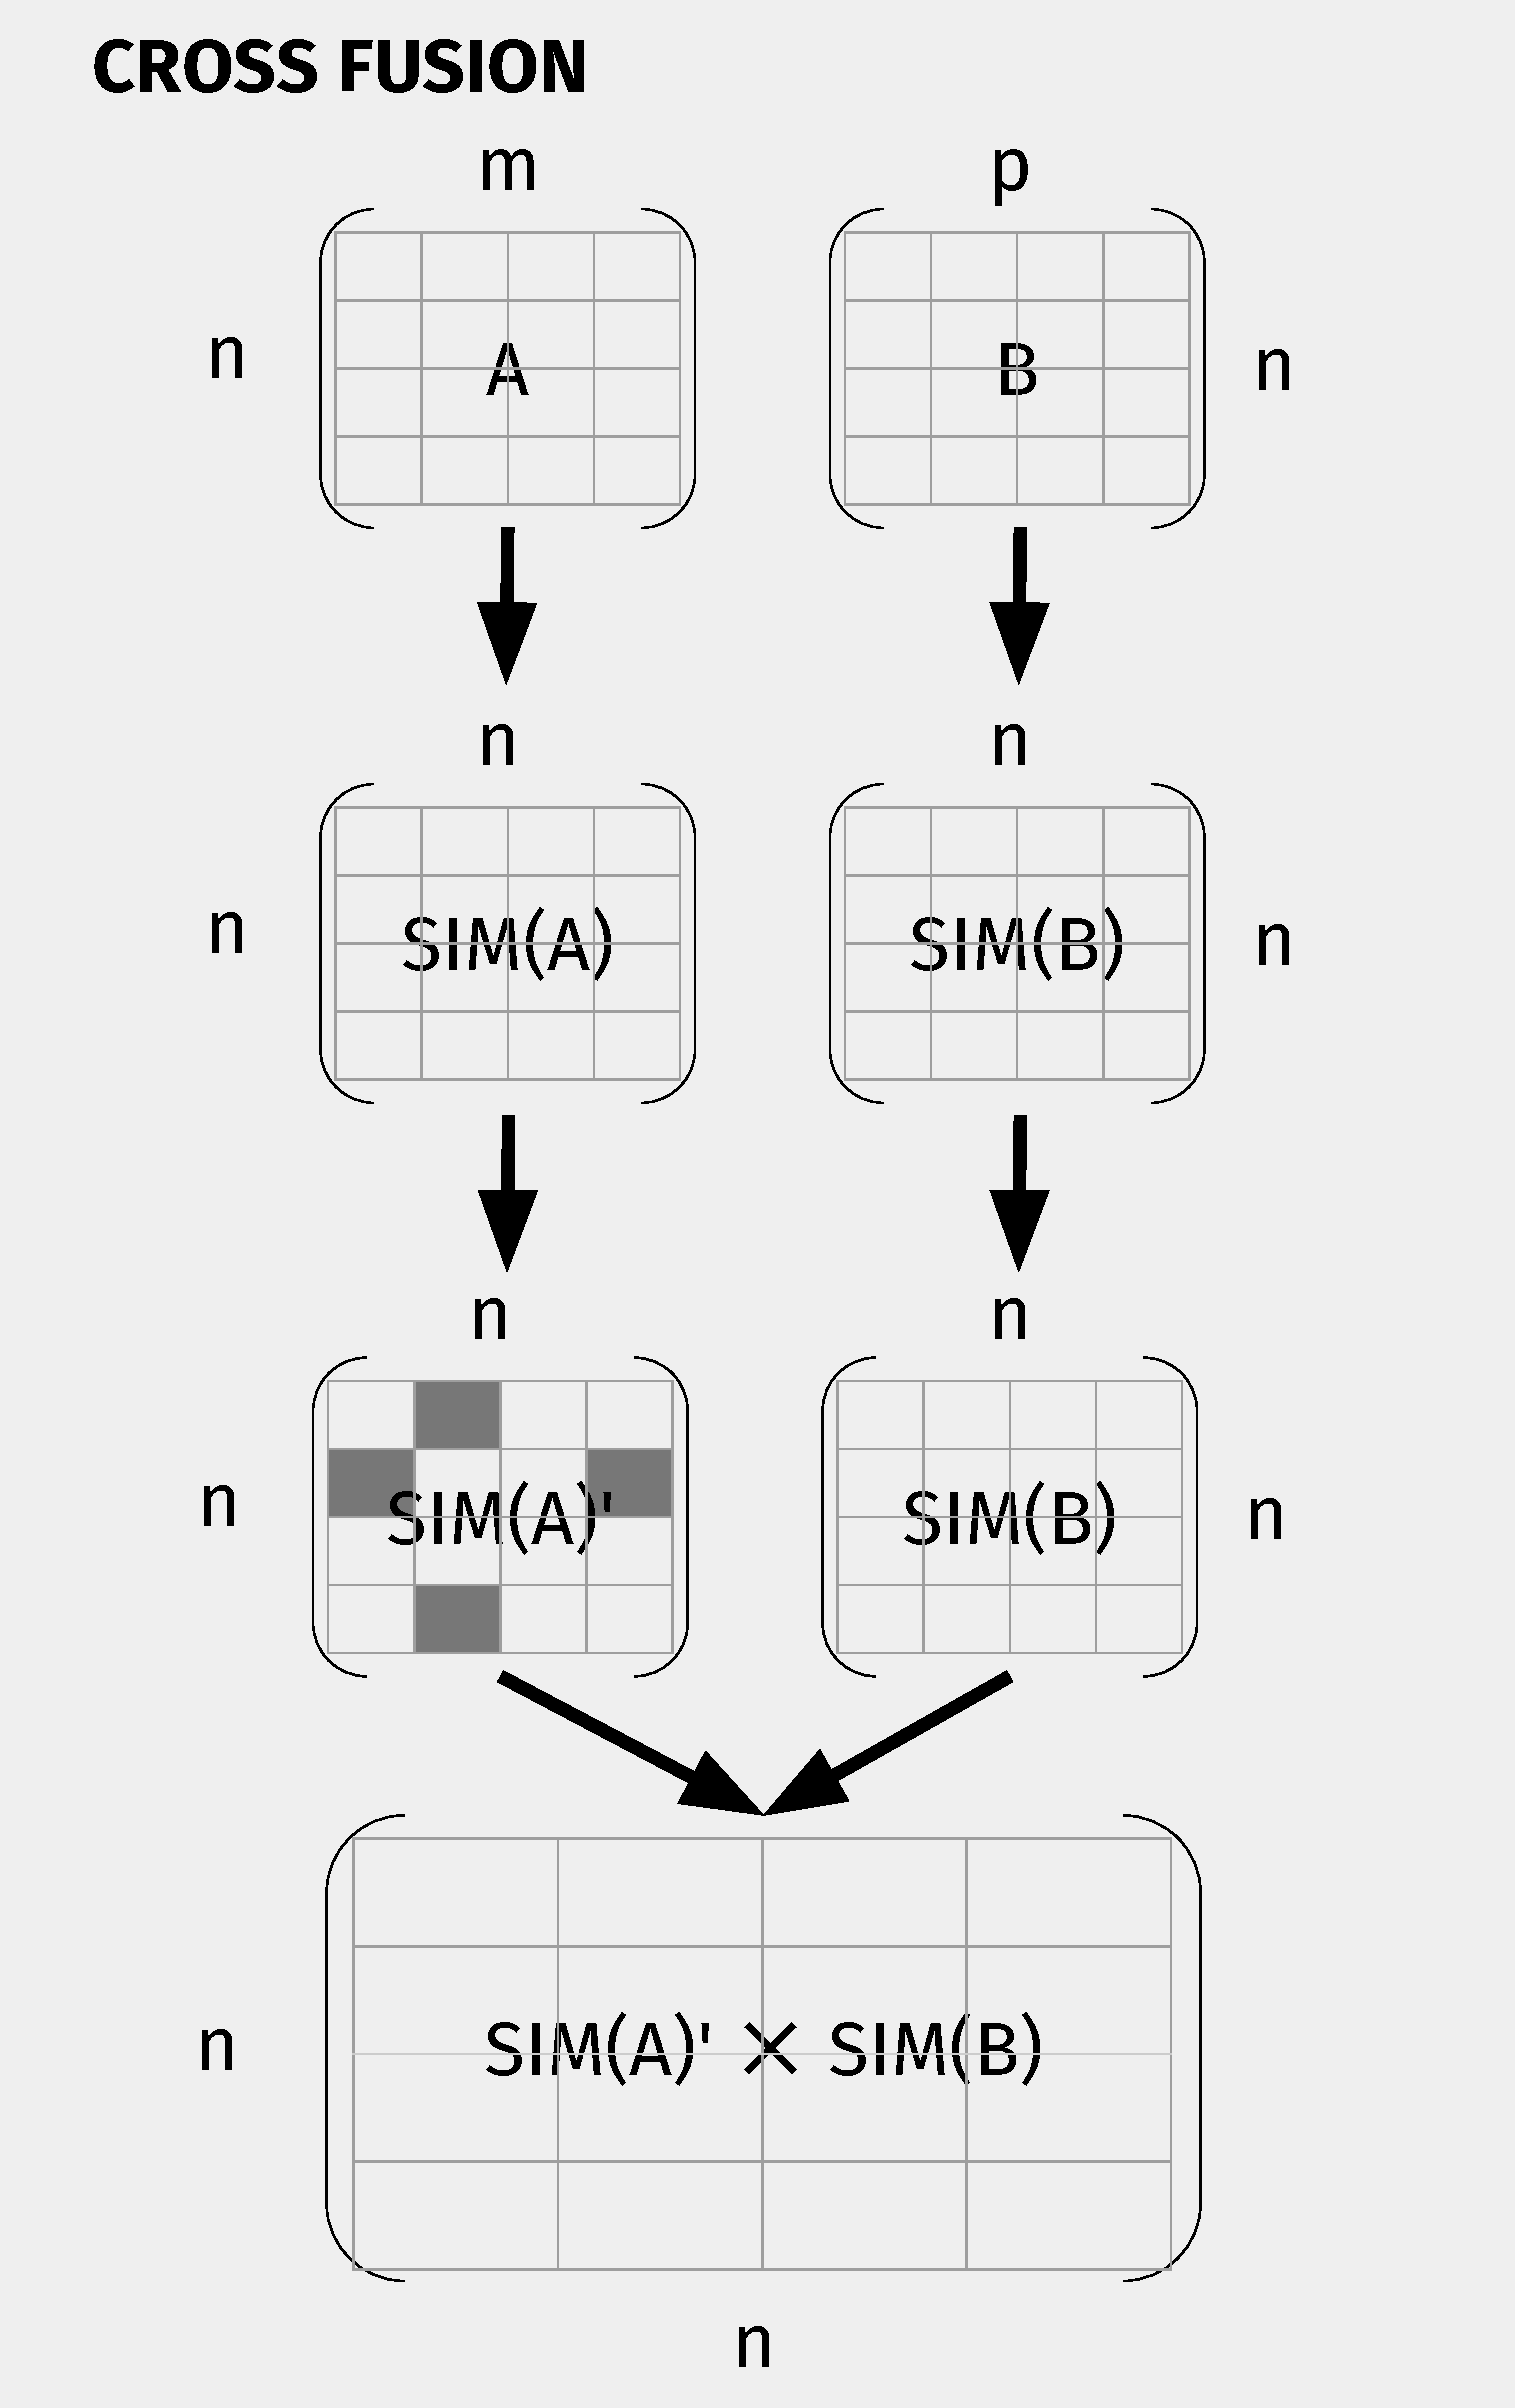
\includegraphics[width=0.6\linewidth]{images/Chapitre3/xf_diag.pdf}
\caption{Cross fusion for matrices $A$ and $B$. Similarities are computed, the best similarities are selected for $A$ and finally a product is calculated between the similarities of $B$ and the top similarities of $A$.}
\label{fig:xf_diag}
\end{figure}

Figure \ref{fig:xf_diag} shows this cross fusion example, between matrices $\mlex$ and $\msyn$. First, their corresponding similarity matrices $\slex$ and $\ssyn$ are first obtained. Secondly, a  top-nearest neighbors operation is applied, $\mathbf{K}(\slex, \gamma)$, yielding a matrix which contains only the most representative similarities, determined by the parameter $\gamma$. Finally, the cross fusion representation is obtained by computing the product $\mathbf{K}(\slex, \gamma) \times \ssyn$.

Formally, we define the cross fusion function as:
\begin{equation}\label{eq:xfusion}
X_{\gamma}(A,B) = \mathbf{K}(A,\gamma) \times B
\end{equation}

In this case, the $\mathbf{K}(\cdot)$ function takes the top-$\gamma$ closest words (columns) to each word (lines) while the rest of the values are set to zero. As noted before, matrices $A$ and $B$ are usually similarity matrices. While $A$ is always required to be a square filtered similarity matrix, $B$ may be also a plain term-feature matrix, as we describe in the following paragraphs.
The sole requirement is that the number of columns of $\mathbf{K}(\cdot)$ should be equal to the number of rows of $B$.

Cross fusion aims to bridge the semantic gap between two modalities by using the most similar neighbors as proxies to transfer valuable information  from one modality onto another one. Usually, the result of a cross fusion is combined with the previous techniques, early and late fusion. In this work we perform  experiment in that sense.

\paragraph{Hybrid Fusion}
We may leverage the advantages of the previous three types of fusion techniques by combining them once more in a hybrid setting. As described in \cite{AtreyHEK10,yu2014informedia}, the main idea is to simultaneously combine features at the feature level, i.e., early fusion, and at the same semantic space or decision level. Nonetheless, they define a specific type of hybrid fusion. In this chapter, we adopt a looser definition of hybrid fusion. That is, we perform a hybrid combination of features by leveraging the aggregation of the fusion strategies described before. 

Having said that, here we distinguish three levels of hybrid fusion that we employ in our experiments during the Chapter \ref{chap:wsd}. 

 \begin{enumerate}
\item \textbf{First Degree Fusion}: we  consider the  three elementary fusion techniques described before (early fusion, late fusion, cross fusion) by themselves.  This level of fusion serve as the baseline we set to surpass in order to show the efficacy of the representation feature space found through fusion techniques.
As an example, we may obtain a first degree representation matrix by performing an early fusion between the lexical matrix and the syntactical features matrix: $E(M^{L}, M^{S})$. 

We note that we distinguish two types of cross fusion operators: \textbf{Cross Feature Fusion} ($X_F$) and \textbf{Cross Similarity Fusion} ($X_S$). The former combines a similarity matrix with a feature matrix, e.g., $X(\slex, \msyn)$. The latter joins a similarity matrix with another similarity matrix, for example $X(\ssyn, \slex)$. %Indeed, $X_S$ has the same configuration as the cross fusion presented before. We rename it to distinguish against the $X_F$ configuration. 
The intuition behind cross feature fusion $X_F$ is that the rich information from the first input matrix can be transferred directly to a representation without the need of obtaining its similarity matrix beforehand. We denote them \textit{feature} and \textit{similarity} to refer to the fact that the first one uses simply a feature matrix and the second requires some knowledge from the data, in this case the similarity between terms.

\item \textbf{Second Degree Fusion}: in this level we  begin with the recombination of the outputs of the previous two levels. Namely, this procedure  yields a combination of "second-degree" among fusion methods. Indeed, we introduce four types of second degree fusions employed in the following list. Each one is illustrated with an example:


\begin{enumerate}

\item \textbf{Cross Feature Early Fusion} ($X_FEF$): consists on the cross feature fusion ($X_F$) of two inputs, a similarity matrix, and the output of an early fusion. For example the operation $X_F(\sstd, E(\mlex, \msyn))$ implies the $X_F$ of the similarity matrix $\sstd$ with the early fusion of matrices $\mlex$ and $\msyn$.

% %
\item \textbf{Cross Feature Similarity Fusion} ($X_FX_SF$): entails the cross feature fusion ($X_F$) of two elements, the output of a cross similarity fusion ($X_S$), and a term-feature matrix. For example, the operation $X_F(X_S(\sstd, \ssyn), \mstd)$ is the cross feature fusion ($X_F$) of a cross similarity fusion ($X_S$), the late having similarity matrices $\sstd$ and $\ssyn$ as inputs, and a standard features matrix $\mstd$.

%
\item \textbf{Early Cross Feature Fusion} ($EX_FF$):  this operation consists on the early fusion of a feature matrix with the output of a cross similarity fusion. As an example, the operation $E(\mstd,X_F(\slex, \mstd))$ computes the early fusion of matrix $\mstd$ with the result of a $X_F$ with $\slex$ and $\mstd$ as operands. 
%

\item \textbf{Late Cross Feature Fusion} ($LX_FF$): this fusion implies the late fusion of a feature matrix with the output of a cross feature fusion. For example, the fusion $L(\mstd, X_F(\sstd, \mstd))$ describes a late fusion between the feature matrix $\mstd$ and the cross feature fusion among $\sstd$ and $\mstd$.
\end{enumerate}

% A second-degree fusion would be an early fusion of the lexical feature matrix with a cross fusion, expressed as $E(M^{L}, \allowbreak X(S^{T}, M^{T}))$.   
\item \textbf{Higher-Degree Fusion}: in this last level we follow a similar approach to the previous level by combining the output of the second-degree fusion level multiple times (that is, more than two times) with other second-degree fusion outputs. In this level we test the following two fusion operations:
\begin{enumerate}
\item \textbf{Early Late Cross Feature Fusion} ($ELX_FF$): As an example for this fusion, the operation $E(\mstd, \allowbreak L(\msyn, X(\sstd, \mstd)))$ implies the combination of three fusion operations. From left to right, first we compute the early fusion (first operation) of  matrix $\mstd$, with the result of a late fusion (second operation) between feature matrix $msyn$ and the result of a cross feature fusion, itself having as input matrices $\sstd$ and $\mstd$. Indeed, we perform three operations, an early fusion, a late fusion and a cross feature fusion, thus the name Early Late cross feature fusion of this operator.
\item \textbf{Triple Early Double Late Cross Feature Fusion\footnote{We adopted the \textit{double} and \textit{triple} notation to lighten the explicit name of this fusion operation: Early Early Early Late Cross Feature Late Cross Feature Fusion}}
%Early Early Early Late Cross Feature Late Cross Feature Fusion
 ($EEELX_FLX_F$): althoug it seems complex, this fusion scheme merely consists on the early fusion of the last two operators: $LX_FF$ and $ELX_FF$, with another feature matrix. As an example, the operator  $E(\mlex, E(E(\mstd,  L(\mstd, X(\sstd, \mstd))),\allowbreak L(\mlex, X(\ssyn, \mlex))))$ entails the early fusion of matrix $\mlex$ with the result of the early fusion of $ELX_FF$ with $LX_FF$.
\end{enumerate}

	
%As an example, the equation $E(L(M^{T}, \allowbreak X(S^{T}, M^{T})),  L(M^{L}, X(S^{S}, M^{L})))$  \allowbreak denotes the early fusion between two operations: (1) a late fusion between a lexical-features matrix and a cross fusion, and (2),  another late fusion consisting of a standard-features matrix (this matrix is detailed below)  and a cross fusion. In general, we determine a n-degree fusion empirically. That is to say, we look at the performance of second-degree fusions and try to improve the performance of the systems by recombining the fusion outputs via a n-degree combination. This process is in fact applied during the second-degree fusions also. 
	\end{enumerate}   


%\paragraph{Discussion}             
The fusion operators presented (early, late, and cross fusion) are simple and straight-forward. In total, they have two parameters to control: $a$ in late fusion, controlling the importance for each matrix $A$ and $B$; and $k$, controlling how many top similarities are kept in cross fusion.

As we will see in the experiments carried out in the next chapter, it is the aggregation of several of these fusion functions, as hybrid fusion operations, that yields interesting results against the use of single features or independent fusion operators. This is in line with other relevant research \cite{Ah-PineCC15}. We consider early fusion, the simple concatenation, a baseline to the rest of fusion aggregations we perform. 

Fusion techniques also have downsides. As said before, certain  operators densify the feature-space matrix but at the same time the number of dimensions grow considerably (with the early fusion operation). Additionally, to the increment of density, the number of features represent an important challenge computationally. 
%We address these concerns on the following chapter.

Before getting into the experimentation details, in order to make our hypergraph linguistic resource concrete, we present the process to obtain such a representation from a raw corpus, namely the English Wikipedia. In other words, we instantiate our model with a Wikipedia-based corpus in order to better understand the characteristics proposed. To get there, we first need a syntactically parsed Wikipedia corpus. In the following section, the method we describe first extracts text from the corpus and then analyses it to create a Syntactically Annotated English Wikipedia Dump (SAEWD). From there, we detail the steps we carried out to store it as the proposed language network (represented as a hypergraph incidence matrix accompanied by complementary metadata information regarding the meaning of each vertex and hyperedge). 



\section{Proof of Concept: Wikipedia-based Corpus as an Enriched Hypergraph}
%In order to have a working dataset, we first built an application that process and parse any input corpus. We describe its properties, its inputs, the information extracted, as well as the output generated by the software.

In order to materialize our proposed linguistic model, we need to first create a chain of applications that will extract text from a semi-structured body of text, tokenize it, parse it to extract the syntactic trees the model requires, and then store in order to be used by a NLP application. In this section we describe this process, implemented as an application that takes a corpus as input and outputs the linguistic resource we introduced in the previous section. In this practical example, we use the English Wikipedia corpus as the source for our resource.

%\subsection{Related Parsed Dumps}
%Today, the broad reach of Wikipedia in Text Mining (TM) and Natural Language Processing (NLP) research  is indisputable. Several recent approaches and tools have  been conducted based on the explicit and implicit knowledge contained in it. Certainly, Wikipedia provides a common ground for researchers and developers to test and compare their results.

The online encyclopedia Wikipedia\footnote{\url{https://en.wikipedia.org}} has been used as a source of valuable data as well as a common background corpus to perform experiments and compare results for diverse NLP/TM related tasks. For example, concerning the first case, in the area of Information Extraction, Wikipedia's infoboxes structured information is used in \cite{Wu2010} as a valuable resource to complement and improve their open IE system. Along the same line, \cite{charton2010}  extracted metadata from Wikipedia while leveraging its internal structure in order to produce a semantically annotated corpus. Moving on to the Information Retrieval field, features extracted from Wikipedia can also help to better predict the performance of a query  \cite{katz2014} in a given  corpus.  In the second case, as a background collection for experiments, a document-aligned version of English and Italian Wikipedia has been used to determine the quality between word's translations \cite{vulic2011}.  

Wikipedia, being such a popular resource  already has various off-the-shelf parsed snapshots (or dumps). These parsed dumps allow researchers to focus more into their approaches than into the extraction and transformation of Wikipedia's data.  We briefly describe certain relevant parses found in the literature.   
%



%The already mentioned parsed dump from \cite{ATSERIAS08}
A relevant Wikipedia parsed dump example comes from \cite{ATSERIAS08}. Their work provides a balanced amount of syntactic and semantic information. In short, the dump includes each word's part of speech tag, their dependency relations as well as the output of three different named entity recognition parsers. Additionally, they provide a graph structure that leverages Wikipedia's internal composition alongside its corresponding metadata. Nonetheless, the resource is no longer available on the original URL although it may be obtained through Yahoo's Webscope\footnote{\url{https://webscope.sandbox.yahoo.com/}} datasets library.  In \cite{FLICKINGER10}, they perform a deep parse analysis is performed to provide detailed syntactic and semantic information. The authors leverage a previously manually annotated portion of the English Wikipedia. They extract a grammar from this portion and also train a statistical model  to automatically parse the rest of Wikipedia. Even though the parse offered is deep and rich in details, the annotation labels, as well as the corpus output format, may not be convenient and easy to use because of its complexity and particular nature. \cite{SchenkelSK07}  released a purely semantic XML parse that links WordNet concepts to Wikipedia pages. They focus greatly on cleaning and pretreating Wikipedia. In this paper we do not focus as much into the cleaning of Wikipedia as already available tools can solve the task quite well for non-specific needs. 
Finally, there are certain Wikipedia dumps that offer the raw cleaned text without any extra subsequent parsing or analysis. Such is the case of the corpus made available by \cite{westbury2010}. This corpus makes  use of the \textit{WikiExtractor} script  \cite{Attardi2015} to clean the Wikipedia dump.
  
  
Although the existing parses and dumps already satisfy numerous specific research needs, they have certain limitations that drove us to build our own resource: the Syntactically Annotated English Wikipedia  Dump (SAEWD). Specifically, we address the following shortcomings: the lack of constituents-based tree information, the complex output formats, the limited online access and the absence of the tools used (i.e., the source code) to create the annotated corpus. In SAEWD we include the complete parse tree information for each word provided by well-known parsing tools. We store the extracted information in a simple and already existing output format. Additionally, we give open access to the parsed dump and we share our source code with the community. The code allows anyone (with programming skills) to  apply our processing pipeline and build their own particular Wikipedia parse or even to parse other text collections. Finally, we present and provide a hypergraph linguistic network for fast NLP/TM experimentation. Indeed, SAEWD aims to be used as a stepping stone for a standard Wikipedia parsed version for the largest possible set of tasks in future research. 

SAEWD uses widely known English language parsing tools, namely those included in the Stanford CoreNLP suite.  Aside from being accessible and regularly maintained, it provides a common set of labels (Universal Dependencies\footnote{\url{http://universaldependencies.github.io/docs/}}) used by numerous NLP and TM experiments. Regarding SAEWD output's format, we believe that the file format we use, which follows  that of \cite{ATSERIAS08}, allows for fast reading and simple interpretation. Among other syntactical information, we provide the constituents parse branch for each word (explained in detail in Section \ref{text:description}). 
Constituent's paths, and hence chunk's production rules, have been proved useful as a complement feature to classic text representations \cite{sagae2009,Bergsma2012,Massung2013}. 
%This information is commonly missed by most Wikipedia parses. It may be due to the fact that it may not be easy or clear to use the constituents nodes information; or may be because storing a tree branch is not as straightforward as stocking a single relationship type label, as is the case of a dependency parse.

Furthermore, we propose a hypergraph linguistic representation. Over the past few years, research on the NLP domain has been focusing on novel techniques that take advantage of the characteristics of language networks to achieve new and interesting results \cite{Mihalcea2011}. That is why, in addition to SAEWD, we also propose, as a proof of concept, a hypergraph representation that stores certain information found in a SAEWD in a practical way that allows for fast and effortless data extraction. This hypergraph can be indeed considered as a Linguistic Network \cite{Choudhury09}.  It aims to facilitate the implementation of graph-based approaches by allowing researchers to jump directly into the algorithm development stage. We use a sub-sample of the Wikipedia corpus consisting of articles related to Natural Language Processing and Text Mining. 
% Our parsed dump,  the source code used to generate it, the network and its metadata will be online and available for LREC 2016.

%In the following sections we describe the steps we undertook to transform a Wikipedia dump into SAEWD (Section 2), we give a detailed account of the contents of SAEWD and the format in which we stored the parsed information (Section 3), then we explain the characteristics of our proposed network structure (Section 4). % Lastly, we present our final comments on the nature of the work done as well as possible future work perspectives.




\begin{figure}[t]

	\centering
	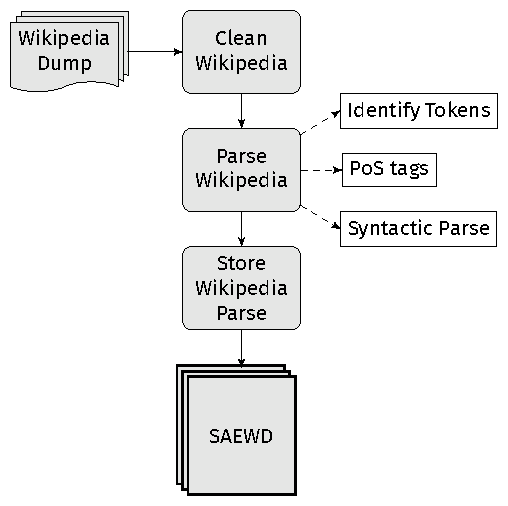
\includegraphics[scale=.8]{images/Chapitre7/flow_chart.pdf}
	\caption{The tree steps we took to build SAEWD.}
	\label{fig:flow}
%TODO change figs to Chapter4 folder!
\end{figure}

\subsection{Construction of SAEWD}
The three main steps we followed to build SAEWD are presented in Figure \ref{fig:flow}. Briefly, we have one input, which is the Wikipedia dump and one output which is the parsed snapshot. In the following we provide a detailed description of each of the process. 

 
We begin the construction of the parsed corpus with the Wikipedia dump XML file obtained from the Wikipedia database\footnote{\url{https://dumps.wikimedia.org/enwiki}} from early November 2014. This dump  contains around 4.7 million article pages\footnote{We kept all articles available in the Wikipedia dump.}. As shown in Figure \ref{fig:flow}, we apply the following processing steps in order to yield the final parsed version.
 
\subsubsection{Cleaning Wikipedia} First, we discard Wikipedia's  tables, references and lists, markup annotations and HTML tags with the \textit{WikiExtractor} \cite{Attardi2015}  script. 
We used this tool to clean and split the content of the original XML file into 429 folders each one containing 100 files of approximately 300 kB. These files contain a certain number of complete Wikipedia articles which is automatically determined by WikiExtractor  according to the maximum possible size assigned for each file, 300 kB in our case, thus the number of articles in each file may vary. We decided to use numerous files as well as a small size to easily read their content into memory while parsing. Having multiple small files also makes it easier to handle the multi-threading aspect of our parsing tool.
We kept WikiExtractor's original folder nomenclature which assigns to each one of them a sequence of letters sorted lexicographically\footnote{We have folders named \textit{AA}, \textit{AB}, \textit{AC} and so on.}. The files containing the cleaned text is simply named \textit{wiki\_XX} where  \textit{XX} goes from 00 to 99, as we have 100 files per folder. 
It is important to note that the Wikipedia articles' titles themselves are not sorted in any specific way, as it was not in the interest of our research to have them ordered. 
Inside each cleaned file, besides the article's text, WikiExtractor keeps the original article's URL as well as its unique Wikipedia ID within an XML-like label that also doubles as  article separator. 

\subsubsection{Parsing Wikipedia} Next, once the Wikipedia dump had been cleaned, we use the Stanford CoreNLP\footnote{\url{http://nlp.stanford.edu/software/corenlp.shtml}} \cite{manning2014} analysis tools to parse all the file texts produced during the previous step. As a part of our processing pipeline, we first perform  sentence segmentation, word tokenization and lemmatization. Below, we briefly describe each of the extracted attributes. We also exemplify them in detail in Section \ref{text:description}.
\begin{itemize}
\item \textbf{PoS tagging}: we obtain the grammatical category of each word, i.e., the part-of-speech tag, using the CoreNLP default tagger, the \textit{left3words} PoS tagging model.

\item \textbf{Constituents parse}:                                                                                                                                                           
the output of this analysis is a rooted tree that represents the syntactic structure of a phrase.                                                                                  
This tree is commonly known as the constituency-based parse tree.                                                                                                                  
For each word, we store its complete path in the constituency tree.
 Specifically, we keep all the nodes of a word's own branch from the root to the word itself.
 We employ the Stanford Shift-Reduce parser.
 This path is transformed into a single line and included in SAEWD. 
\item \textbf{Dependency parse}: this attribute consists on an extracted tree that describes the types of grammatical relations between words, i.e., the dependency-based parse tree. 
The analysis was performed with the Stanford's \textit{Shift-Reduce}  parser.
% This parser is known to perform better than other Stanford parsers.                                  
 %(notably  faster and  with stronger \textit{F1} measure than the previous PCFG parser, although not as accurate as the Recurrent Neural Network system trained with semantic word vectors).
As information representation, we use the basic dependencies scheme, as we wanted to include each one of the possible dependency relations without any collapsing between them.     

\end{itemize} 	
%\section{Parsed files organization}
 Finally, once the parsing process is complete, the parsed files are stored into individual files and thus there are as much parsed files as input Wikipedia cleaned files. The parsed files keep their original name plus the \texttt{parsed} extension, e.g., \texttt{wiki\_00.parsed}. The structure within the files is described in Section \ref{section3.2}. After parsing, we found the statistics shown in Table \ref{tab:corpus_stats}.
 
\begin{table}[t]
\centering
\caption{English Wikipedia dump statistics.}
\label{tab:corpus_stats}
\begin{tabular}{lr}
{\bf Number of tokens}      & 1,889,769,908 \\
{\bf Unique tokens (types)} & 8,761,691 \\
{\bf Number of sentences}   &  84,760,512\\
{\bf Average number of tokens per sentence} & 22.30
\end{tabular}
\end{table}

\subsection{SAEWD Description}\label{text:description}
In this section we describe in detail the characteristics of SAEWD.




\begin{table*}[ht]
\centering
\caption{Extract of a Wikipedia parsed file. The phrase shown is the parse result of the previous example sentence in Figure~\ref{fig:tree_saewd} }
\label{tab:parse}
\noindent\makebox[\textwidth]{%
\begin{tabular}{llllll}
 \multicolumn{6}{l}{\textit{FILENAME wiki\_00.parsed}}                                           \\ \hline
  \textbf{token}   & \textbf{lemma}   & \textbf{POS} & \textbf{constituency}                      & \textbf{head} & \textbf{dependency} \\ \hline
 \multicolumn{6}{l}{\textit{\%\%\#PAGE Anarchism}}                                         \\ \hline
  {$\vdots$}      &      {$\vdots$}   &  {$\vdots$}   &     {$\vdots$}                              &    {$\vdots$}  &     {$\vdots$}       \\  \hline
 \multicolumn{6}{l}{\textit{\%\%\#SEN 25  9}}                                             \\ \hline
						 A       & a       & DT  & NP\_22,S\_97                      & 3    & det        \\ %\cline{2-7} 
                         great   & great   & JJ  & NP\_22,S\_97                      & 3    & amod       \\ %\cline{2-7} 
                         brigand & brigand & NN  & NP\_22,S\_97                      & 4    & nsubj      \\ %\cline{2-7} 
                         becomes & become  & VBZ & VP\_44,S\_97                      & 0    & root       \\ %\cline{2-7} 
                         a       & a       & DT  & NP\_18,NP\_20,VP\_44,S\_97        & 6    & det        \\ %\cline{2-7} 
                         ruler   & ruler   & NN  & NP\_18,NP\_20,VP\_44,S\_97        & 4    & xcomp      \\ %\cline{2-7} 
                         of      & of      & IN  & PP\_57,NP\_20,VP\_44,S\_97        & 9    & case       \\ %\cline{2-7} 
                         a       & a       & DT  & NP\_18,PP\_57,NP\_20,VP\_44,S\_97 & 9    & det        \\ %\cline{2-7} 
                         Nation  & nation  & NN  & NP\_18,PP\_57,NP\_20,VP\_44,S\_97 & 6    & nmod       \\ %	\cline{2-7} 
\hline 
      
\end{tabular}}
\end{table*}

% Please add the following required packages to your document preamble:
% \usepackage{multirow}
% \usepackage{graphicx}
\begin{table*}[ht]
\centering
\resizebox{\textwidth}{!}{%
\begin{tabular}{cl|cccc|cccc|c}
\multirow{2}{*}{\textbf{PoS Tag}} & \multirow{2}{*}{\textbf{Token}} & \multicolumn{4}{c}{\textbf{NP}} & \multicolumn{4}{c}{\textbf{DEP}} & \multicolumn{1}{l}{\textbf{SEN}} \\ 
 &  & \multicolumn{1}{c}{$ \text{NP\_22}_1 $} & \multicolumn{1}{c}{$ \text{NP\_20}_1 $} & $ \text{NP\_18}_1  $& \multicolumn{1}{c}{$ \text{NP\_18}_2 $} & nsubj\_become & xcomp\_become & nmod\_ruler & \multicolumn{1}{c}{amod\_brigand} & \multicolumn{1}{l}{$ \text{~~S}_1 $} \\ \cline{1-11} 
\multirow{3}{*}{\textbf{NN}} & \multicolumn{1}{l|}{brigand} & 1 &  &  &  & 1 &  &  & & 1 \\
 & \multicolumn{1}{l|}{ruler} &  & 1 & 1 &  &  & 1 &  &  & 1 \\
 & \multicolumn{1}{l|}{nation} &  & 1 &  & 1&  &  & 1 &  & 1 \\ \hline
\textbf{VB} & \multicolumn{1}{l|}{becomes} &  &  &  &  &  &  &  & & 1 \\ \hline
\textbf{JJ} & \multicolumn{1}{l|}{great} & 1 &  &  &  &  &  &  & 1 & 1 \\ \hline
\end{tabular}
}
\caption{Brief example of the linguistic network incidence matrix of the previous used phrase. On the left side, as on the top, we can see the metadata we store for each word (rows) and each column (hyperedges). We omit the rest of the words from the example phrase for brevity.  }
\label{ref:incidence}
\end{table*}

\paragraph{Constituency parse storage in detail}
%The  result from the constituency parse is not as straightforward to store as the other kinds of parses, i.e., the output is  a deeper tree structure than that of a dependency parse. Thus, we believe that the storage of this information in SAEWD requires a more in detail explanation. 
%In this subsection, we will describe how we stock the information concerning  the phrases' constituents. 

We will use an example to better explain the storage of the constituency-based parse tree. In Figure \ref{fig:tree_saewd} we can see the constituency parse of the phrase  \textit{A great brigand becomes a ruler of a Nation}. On the bottom of the figure, we observe the constituent's path (or branch), of the words \textit{brigand} and \textit{Nation}. As in any tree structure, each leaf node has a defined path from the root node to itself. In this example, the leaf containing the noun \textit{brigand} 
%(PoS tag \textit{NN})
 follows the bottom-up path \textit{NP22}$\rightarrow$\textit{S97}. \textit{Brigand's} parent node is a Noun Phrase (NP) node which in turn comes from the root of the tree, the Sentence node \textit{S}. We assign to each phrase chunk an identifier (22 and 97 in this case) in order to distinguish them according to their building elements as specified by the grammar rule used.
  In other words, a phrase chunk, e.g., a NP, a Verbal Phrase (VP), a Prepositional Phrase (PP), or other chunk defined by the grammar in CoreNLP, may be built from different types of PoS tags. Thus, again from Figure \ref{fig:tree_saewd}, we see that the sentence \textit{S97} is  built both from a NP and a VP chunk. 
 In a similar way, the noun phrase \textit{NP18} is produced by a determinant (DT) and a noun (NN), while  \textit{NP22} is generated by a determinant, an adjective (JJ) and a noun.
  The identification digits are obtained from the hash code that represents each chunk object inside our Java application. For each phrase-chunk tree node, we keep the last two significative figures produced by the \texttt{hashCode}\footnote{Java \texttt{hashCode} function description: \url{https://en.wikipedia.org/wiki/Java\_hashCode\%28\%29}} Java method.
%\begin{figure}[]
%\resizebox{\linewidth}{!}{%
%\begin{forest} 
%[S97
%	[NP22 [DT [A, blue text]] [JJ [great, blue text]] [NN [brigand, blue text]]]
%    [VP44 [VBZ [becomes, blue text]]
%      [NP20
%        [NP18 [DT [a, blue text]] [NN [ruler, blue text]]]
%        [PP57 [IN [of, blue text]]
%          [NP18 [DT [a, blue text]] [NN [Nation, blue text]]]]]]]
%	\node [draw,fill = blue!20,text width=21em] at (1.5,-6.8) (sparse) {\textbf{brigand} (NN): NP22$\rightarrow$S97 \\ \textbf{Nation} (NN): NP18$\rightarrow$PP57$\rightarrow$NP20$\rightarrow$VP44$\rightarrow$S97};
%\end{forest}
%}

%\caption{Constituency tree for the phrase \textit{{A great brigand becomes a ruler of a Nation}.}
%% On the bottom, we can see the bottom-up path stored for the words \textit{brigand} and \textit{Nation}.
%}
%\label{fig:tree_saewd}
%\end{figure}

\begin{figure}
\centering
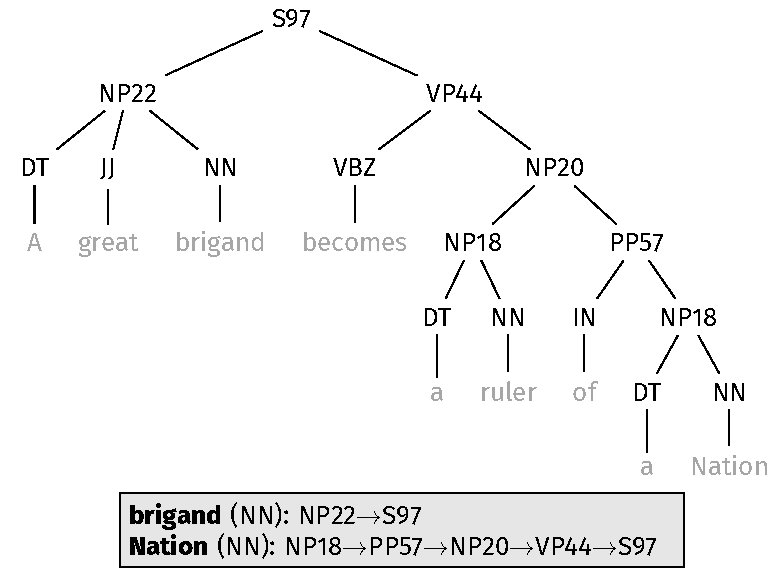
\includegraphics[width=0.8\linewidth]{images/Chapitre3/trees/tree_saewd.pdf}
\caption{Constituency tree for the phrase \textit{A great brigand becomes a ruler of a Nation}. On the bottom, we can see the bottom-up path stored for the words \textit{brigand} and \textit{Nation}.}
\label{fig:tree_saewd}
\end{figure}
 


As another example, the noun \textit{Nation} has the following bottom-up constituency path: \textit{NP18}$\rightarrow$\textit{PP57}$\rightarrow$\textit{NP20}$\rightarrow $\textit{VP44}. Indeed, the string \texttt{NP\_18,PP\_57,NP\_20,VP\_44,S\_97}, originating from the previously described path,  is the information we keep about the constituency parse for each token in the Wikipedia dump.



\paragraph{Annotation scheme}\label{section3.2}
To store the parsed text we use a scheme  inspired by that used in \cite{ATSERIAS08}. The format can be considered as a regular Tab Separated Values file  (extension tsv), with additional metadata tags. An extract from a parsed file can be observed in Table \ref{tab:parse}. 

The file includes two headers: the first one simply indicates the name of the current parse file; the second one contains the names that describe each column. The tags and columns our parsed dump contains are the following:
\begin{itemize}
\item Metadata tags:
\begin{enumerate}
\item {FILENAME}: indicates the original file used to extract the current parse, 
\item {\%\%\#PAGE}: denotes a new Wikipedia article, as well as its title, 
\item {\%\%\#SEN}: marks the beginning of a new sentence. It is followed by two integers: (1) the number of the current sentence, and (2), the number of tokens in the sentence.

\end{enumerate}

\item Parse columns for each token:
\begin{enumerate}
\item Token: the token itself,
\item Lemma: the token the canonical form,
\item POS: its part of speech tag,
\item Constituency: the bottom-up constituency path described before,
\item Head: the head index of the dependency relation the current token belongs to,
\item Constituency: the name of the grammatical relationship this token participates in as a dependent.
\end{enumerate}
\end{itemize}

Using the example phrase introduced before (Table \ref{tab:parse}), the token \textit{becomes} has \textit{become} as lemma, it is a verb, thus it has \textit{VBZ} as PoS tag, its constituency path is \textit{VP\_44,S\_97}, so it belongs to the verb phrase {VP44} which in turn comes from sentence {S97}. Finally, \textit{becomes}, being the main verb, is in this case the grammatical root of the sentence and its head is by convention determined as  zero. 

\subsection{Enriched Wikipedia-based Hypergraph}

Once SAEWD is saved to disk, we leverage its information by building a linguistic network by connecting tokens according to their interaction within the Wikipedia corpus. Given the large size of the Wikipedia corpus, we chose a sample of it to illustrate our proposed representation. We randomly selected around 200 thousand articles. %We store the incidence matrix (which is in fact a sparse matrix) on disk as a \textit{Matrix Market} format file. The metadata is stored as \textit{JSON} files. Both formats allow for an easy data lecture.


%\subsection{Enriching the Wikipedia Hypergraph with Fusion Techniques}
%

We focus now on the combination of the linguistic features contained in the model to obtain a more diverse, enriched, and less sparse representation. In this subsection, we present a practical example of what are the differences between each the three essential fusion operators (early, late and cross fusion)  and with respect to using single features independently. For sake of clarity, we focus on two types of linguistic information: lexical (with a context window  of +2-2 around each word) and syntactic (using  dependency relations).

The goals of this example are to show how the type of context affects the semantic relatedness of a given word, to get a glimpse of how heterogeneous features get combined into a single enriched representation ideally allowing us to get more knowledge about a given term, and finally, discover how the sparsity is alleviated by combining two different matrices together, especially using the late and cross fusion techniques. 

The example consists in presenting the top 5 most similar words of the word \textit{priest} according to different representation spaces. These representation spaces are obtained using five representation matrices: the lexical features matrix ($\mlex$),  the syntactic features matrix ($\msyn$), the early fusion matrix $E(\msyn,\mlex)$, the late fusion matrix ($L_{0.5}(\ssyn,\slex)$), and finally two cross fusion matrices ($X_F(\ssyn,\mlex)$ and $X_F(\slex,\msyn)$). We  report the sparsity level of each matrix (percentage of zero values in the matrix) obtained. 

The procedure to obtain said similar words consist in calculating a cosine-similarity matrix for each of the five fusion representations. In some cases, as in late fusion and cross fusion, this step is implicit as in this example, these operators already require the computation of similarity matrices (see Equations \ref{eq:late-fusion} and \ref{eq:xfusion}).

The  most similar terms to the target word can be seen in Table \ref{tab:priest}. We note that in this example we are not interested in determining the quality of the semantic related words discovered with each representation space. Even more, it seems hard to determine the semantic-relatedness quality of these similar (\textit{similar} in the sense of cosine similarity) words. Still, we can say that, as expected, the words seem to be semantically related in a large sense.

As discussed by \cite{LevyG14}, lexical features seem to give words that are semantically related in a larger sense, in this example, religion related terms. On the other hand, dependency based relations similarities tend to discover functional words or words that are of the same \textit{semantic type}.
With respect to early and late fusion, while the similar words found are already known, we discover new terms that were until now unknown which seem to be semantically related, such as \textit{relic} and \textit{seer}. Concerning the cross fusion, in this case cross feature fusion, both transferring from the syntactic to the lexical similarity matrix and the other way around, we see that we also found previously seen words while discovering yet another couple of related words: \textit{monk} and \textit{chorus}. It is also clear how by selecting to transfer information from the syntactic matrix (fifth column) we get functionally related terms (occupations in the church or in a power structure) while on the sixth column (transfer from lexical to syntactic), we get mostly words that correspond to a broader similarity domain.

With regard to alleviating the data sparsity (indicated below the header of each column as the percentage of non-zero values in the matrix) it is quite obvious that by using a similarity matrix we densify the space by means of a matrix multiplication, which is the case of late fusion and cross fusion: we pass from a sparsity of {5.49}\% in the lexical matrix and {4.97}\% in the syntactic matrix to {83.17}\%, {16.75}\% and {13.45}\% in the late fusion and cross fusion matrices, respectively. The large increment of density in the late fusion representation is obviously due to the use of similarity matrices in this operation, which usually tend to be dense matrices.

Furthermore, for the cross feature fusions, while we also employ a similarity matrix, we stay in the same space (same number of dimensions) of the feature matrix, while more than doubling the density of the space at the same time. 

% Please add the following required packages to your document preamble:
% \usepackage{booktabs}
\begin{table}[]
\centering

\begin{tabular}{@{}lllllll@{}}
\toprule
                           & \textbf{\begin{tabular}[c]{@{}l@{}}Lexical\\ Features\\(5.49\%)\end{tabular}}              & \textbf{\begin{tabular}[c]{@{}l@{}}Syntactic\\ Features\\(4.97\%)\end{tabular}}        & \textbf{\begin{tabular}[c]{@{}l@{}}Early\\ Fusion\\(5.23\%)\end{tabular}}                & \textbf{\begin{tabular}[c]{@{}l@{}}Late\\ Fusion\\(83.17\%)\end{tabular}}                 & \textbf{\begin{tabular}[c]{@{}l@{}}Cross\\Early\\ Fusion\\(16.75\%)\\$X(\ssyn, \mlex)$\end{tabular}}   &
                           \textbf{\begin{tabular}[c]{@{}l@{}}Cross\\ Early\\Fusion\\(13.45\%) \\$X(\slex, \msyn)$\end{tabular}}                 \\ \midrule
\multicolumn{1}{c}{priest} & \begin{tabular}[c]{@{}l@{}}priests\\ nun\\ canton\\ sailor\\ burial\end{tabular} & \begin{tabular}[c]{@{}l@{}}monk\\ regent\\ aedile\\ seer\\ meek\end{tabular} & \begin{tabular}[c]{@{}l@{}}sailor\\ regent\\ nuclei\\ nun\\ relic\end{tabular} & \begin{tabular}[c]{@{}l@{}}regent\\ slang\\ seer\\ tutor\\ cradle\end{tabular} & \begin{tabular}[c]{@{}l@{}}vassal\\ regent\\ nun\\ sailor\\ monk\end{tabular} & \begin{tabular}[c]{@{}l@{}}sailor\\ fluent\\ dean\\ nuclei\\ chorus\end{tabular} \\

 \bottomrule

\end{tabular}
\caption{Target word \textit{priest} and its top 5 most similar words using different feature matrices. The sparsity level (percentage of non-zero values) of each representation is shown below the header of each column.}
\label{tab:priest}
\end{table}

%\paragraph{Discussion}
%Concerning the computation time, SAEWD takes around 40 hours to be produced using a general purpose laptop (Intel i7 4700MQ with 4 cores, 8 GB and Linux Mint 17 as operative system). Most of the time is taken by the parsing step. 
%
%We verified the consistency of the corpus built by analyzing a sample of 20 Wikipedia articles. The output of CoreNLP and the information contained in the corpus match.



\section{Conclusion}

In this chapter  we analyzed the state of the art of linguistic network-based approaches to semantic similarity task from a graph-centric point of view. We reviewed the techniques in terms of its graph characteristics, from their structure to the algorithms employed. Among the literature covered, certain non-explored research paths were identified, namely the lack of syntactic data on the networks employed, and therefore, a homogeneous network nature that only allows for relations of a unique type. 

We addressed these paths with the proposition of a fusion enriched hypergraph linguistic model that is able to hold heterogeneous language information while allowing its combination and alleviating the data sparsity.  This structure allows the integration multiple kinds of information and has potential in terms of which algorithms it can be used with. The three levels of contexts we integrated in the model (sentence lexical co-occurrence, dependency function co-occurrence, and constituent-membership co-occurrence) aim to cover distinct levels of semantic relatedness. We noted the challenges of dealing both with textual data sparsity and leveraging the heterogeneity of the hypergraph. To alleviate both concerns, we propose the use of fusion functions, introduced also in this chapter. The structure of the hypergraph is also an important characteristic that we can use to find groups of semantically related words within a corpus. Finally, we presented a materialization of a corpus, a portion of the English Wikipedia, as the linguistic network we proposed.



